\chapter{Mathematische Einschübe}\label{chap: MathematischeEinschübe}
\section{Folgen und Reihen}\label{sec: Folgen_Reihen}
\subsubsection{Folgen}\label{subsec: Folgen}
Eine \textbf{Folge} ist eine geordnete Liste von Zahlen, die entweder komplett angegeben ist oder nach einer bestimmten Regel gebildet wird. Jedes Glied der Folge wird als Element bezeichnet. Folgen können endlich oder unendlich sein. \\ 

\noindent\textit{Beispiel:} Man möchte die Folge $\{1, \frac{1}{2},\frac{1}{4}, \frac{1}{8}, \frac{1}{16}, \cdots \}$ untersuchen. Die Beschreibung in der Klammer lässt aber keinen vollständigen Schluss zu, wie die Folge weitergeht, obwohl dies zunächst so scheint. Daher definiert man die Folge durch $(a_n)_{n \in \Real} = \frac{1}{n}$. Das bedeutet, dass das $n$-te Glied der Folge $\frac{1}{n}$ ist. Nun sind alle Glieder der Folge eindeutig bestimmt. 


\subsubsection{Reihen}\label{subsec: Reihen}
Eine \textbf{Reihe} ist die Summe der Glieder einer Folge. Wenn man die Glieder einer unendlichen Folge addiert, spricht man von einer unendlichen Reihe. Reihen können konvergieren oder divergieren. \\

\noindent \textit{Beispiel:} Die Summe der Glieder der Folge von oben schreiben wir als
\begin{equation*}
    \sum_{n=1}^{\infty} \frac{1}{n^2} = 1 + \frac{1}{4} + \frac{1}{9} + \cdot .
\end{equation*}
Wenn sich die Summe einem endlichen Wert annähert und im Limes diesen Wert annimmt, spricht man von einer \textbf{konvergenten Reihe}. Oszilliert die Summe um einen bestimmten Wert oder wächst unbeschränkt und nimmt daher im Limes keinen endlichen Wert an, nennt man sie \textbf{divergente Reihe}.
\newpage

\section{Polynome}\label{sec: Polynome}
Polynome sind mathematische Ausdrücke, die aus Variablen und Koeffizienten bestehen, verbunden durch Addition, Subtraktion und Multiplikation. Ein allgemeines Polynom $P(x)$ in einer Variablen $x$ hat die Form:
\begin{equation}
P(x) = a_n x^n + a_{n-1} x^{n-1} + \cdots + a_1 x + a_0 = \sum_{k=0}^{n} a_k x^k \mComma
\end{equation}
wobei $a_n, a_{n-1}, \ldots, a_0$ die Koeffizienten sind und $x$ ist die Variable. Der höchste vorkommende Exponent der Variablen im Polynom -- die höchste Potenz von $x$ ist hier $n$ -- wird der Grad $n$ des Polynoms genannt. \\

Polynome haben mehrere interessante Eigenschaften:
\begin{itemize}
    \item \textbf{Addition und Subtraktion:} Polynome können addiert und subtrahiert werden, indem man die Koeffizienten der gleichen Potenzen addiert oder subtrahiert.
    \item \textbf{Multiplikation:} Die Multiplikation von Polynomen erfolgt durch die Anwendung des Distributivgesetzes.
    \item \textbf{Nullstellen:} Die Nullstellen eines Polynoms sind die Werte von $x$, für die $P(x) = 0$ gilt.
\end{itemize}
Polynome sind in vielen Bereichen der Mathematik und der angewandten Wissenschaften von Bedeutung. Sie werden verwendet, um Kurven zu modellieren, in der numerischen Analyse und in der Algebra.

\section{Tupel}\label{sec: Tupel}
Ein Tupel ist eine geordnete Liste von Elementen. Im Kontext von mehrdimensionalen Räumen sind Punkte, eine Verallgemeinerung von Skalaren und werden oft als Tupel dargestellt. Stellen Sie sich ein Tupel als eine feste Reihenfolge von Werten vor. Im Gegensatz zu einer Menge kommt es bei einem Tupel auf die Reihenfolge der Elemente an, und Elemente können mehrfach vorkommen. Hier sind ein paar Beispiele, um das Konzept zu verdeutlichen:\\

\noindent\textbf{2D-Raum (Ebene):} Ein Punkt im zweidimensionalen Raum wird als Paar von Koordinaten $(x,y)$ dargestellt. Das ist ein $2$-Tupel. Zum Beispiel ist $(3,5)$ ein Punkt, wobei $3$ die $x$-Koordinate und $5$ die $y$-Koordinate ist. Der Punkt $(5,3)$ wäre ein anderer Punkt. \\

\noindent\textbf{3D-Raum:} Ein Punkt im dreidimensionalen Raum ist ein Tripel von Koordinaten $(x,y,z)$. Das ist ein $3$-Tupel. Ein Beispiel wäre $(1,2,7)$ oder $(-3,4,-3)$.\\

\noindent\textbf{n-dimensionaler Raum:} Allgemein wird ein Punkt in einem $n$-dimensionalen Raum durch ein $n$-Tupel von Koordinaten $(x_1, x_2, \,\ldots, x_n)$ beschrieben. Jede dieser Koordinaten ist ein Skalar.\\

Ein Tupel von Koordinaten kann keine Richtung vermitteln. Das Tupel beschreibt lediglich einen Ort im $n$-dimensionalen Raum. Zusammenfassend lässt sich sagen, dass ein Tupel eine mathematische Struktur ist, die es ermöglicht, die Koordinaten eines Punktes in einem mehrdimensionalen Raum zu erfassen.

\newpage
\chapter{Vektorrechnung}\label{chapter: Vektorrechnung}
\section{Unterschied zwischen Vektoren und Skalaren}\label{sec: Vektor_vs_Skalar}
In mehrdimensionalen Räumen sind \textbf{Punkte} $P = (x,y,\ldots)$ die Verallgemeinerung von \textbf{Skalaren}. \textbf{Punkte} vermitteln \textbf{keine Richtung} -- sie sind ein $n$-Tupel von Skalaren. Punkte sind „ortsfest“, aber ihre Koordinaten hängen vom gewählten Koordinatensystem ab.

% tikz picture
\begin{figure}[h!]
    \centering
    \begin{minipage}[b]{0.48\textwidth}
        \centering
        \resizebox{\linewidth}{!}{
            \begin{tikzpicture}
                % 1. Draw the horizontal axis
                \draw[->, line width=1.2pt] (-3, 0) -- (9, 0) node[right] {\large $x$};
                % 2. Add the tick marks and labels
                \foreach \x in {-2, 0, 2, 4, 6, 8} {
                    \draw[line width=1.2pt] (\x, -0.15) -- (\x, 0.15);
                    \node[below=5pt] at (\x, 0) {\x};
                }
                % 3. Draw the solid blue point at x=3
                \node[circle, fill=pointblue, inner sep=2.8pt] at (3, 0) {};
                % 4. Add the label above the point
                \node[above=7pt, color=pointblue] at (3, 0) {\LARGE $x=3$};
                \node[color=black] at (-2, 3.6) {\Huge $\Real^1$};
            \end{tikzpicture}
        }
        \caption{Ein Punkt auf dem Zahlenstrahl ($\Real^1$), der die Gleichung $x = 3$ darstellt.}
    \end{minipage}
    \hfill 
    \begin{minipage}[b]{0.48\textwidth}
        \centering
        \resizebox{\linewidth}{!}{
            \begin{tikzpicture}
                % 1. Draw the axes
                \draw[->, line width=1.2pt] (-3, 0) -- (7, 0) node[right] {\large $x$};
                \draw[->, line width=1.2pt] (0, -1.5) -- (0, 2.8) node[above] {\large $y$};
                % 2. Add the tick marks and labels
                \foreach \x in {-2, 0, 2, 4, 6} {
                    \draw[line width=1.2pt] (\x, -0.15) -- (\x, 0.15);
                    \ifnum\x=0
                        \node[below left=2pt] at (\x, 0) {0};
                    \else
                        \node[below=5pt] at (\x, 0) {\x};
                    \fi
                };
                \foreach \y in {-1, 1, 2} {
                    \draw[line width=1.2pt] (-0.15, \y) -- (0.15, \y);
                    \node[left=5pt] at (0, \y) {\y};
                };
                % 3. Draw the solid blue point
                \node[circle, fill=pointblue, inner sep=2.5pt] at (4,2) {};
                % 4. Add the label above the point
                \node[anchor=south west, color=pointblue] at (4,2) {\Large $P(4, 2)$};
                \node[color=black] at (-2, 3) {\huge $\Real^2$};
            \end{tikzpicture}
        }
        \caption{Ein Punkt in der kartesischen Ebene ($\Real^2$) an den Koordinaten $(4, 2)$.}
    \end{minipage}
\end{figure}

\begin{rememberbox}[]{Definition Vektor}
    \textbf{Vektoren} zeichnen sich im Gegensatz zu einem Skalar dadurch aus, dass sie eine \textbf{Länge} und eine \textbf{Richtung} haben. Vektoren haben keinen festen Start- und Endpunkt und sind damit nicht \gDQ{ortsfest}. Vektoren können über die Vorschrift 
    \begin{equation}
        \mathrm{Vektor} = \mathrm{Endpunkt} - \mathrm{Anfangspunkt}
    \end{equation}
    generiert werden. Ein Vektor vermittelt somit die \textbf{Verschiebung} des Anfangspunktes A zum Endpunkt E und wird auch als $\ivec{AE}$ notiert. 
\end{rememberbox}
Unterschiedliche Start- und Endpunkte können demnach dieselben Vektoren erzeugen. Im Beispielbild rechts sind der blaue Vektor $\ivecS{r}{1}$ und der rote Vektor $\ivecS{r}{2}$ ident, $\ivecS{r}{1}=\begin{psmallmatrix} 2 \\ 1 \end{psmallmatrix} = \ivecS{r}{2}$, obwohl sie von unterschiedlichen Start- und Endpunkten erzeugt wurden. Die Koordinaten eines Vektors hängen ebenso vom Koordinatensystem ab.
\begin{figure}[h!]
    \centering
    \resizebox{0.7\linewidth}{!}{
    \begin{tikzpicture}
    \definecolor{pointblue}{HTML}{004A8F}
    % 1. Draw the horizontal axis
    \draw[->, line width=1.2pt] (-3, 0) -- (9, 0) node[right] {\large $x$};
    \draw[->, line width=1.2pt] (0, -1.5) -- (0, 4.5) node[above] {\large $y$};
    % 2. Add the tick marks and labels
    % A 'foreach' loop is used to place them at regular intervals.
    \foreach \x in {-2, 0, 2, 4, 6, 8} {
        % Draw thick vertical lines for the ticks.
        \draw[line width=1.2pt] (\x, -0.15) -- (\x, 0.15);
        % Place the corresponding number below each tick.
        \ifnum\x=0
            \node[below left=2.1pt] at (\x -0.2, 0) {\x};
        \else
            \node[below=5pt] at (\x, 0) {\x}; 
    \fi
    };
    % small ticks
    \foreach \x in {-1, 1, 3, 5, 7} {
        % Draw small vertical lines for the ticks.
        \draw[line width=1.0pt] (\x, -0.1) -- (\x, 0.1);
    };
    \foreach \y in {-1, 1, 2, 3, 4} {
        % Draw thick lines for the ticks.
        \draw[line width=1.2pt] (-0.15, \y) -- (0.15, \y);
        % Place the corresponding number below each tick.
        \ifnum \y=0
        \else
            \node[left=5pt] at (0, \y) {\y}; 
        \fi
    };
    % small ticks
    \foreach \y in {-0.5, 0.5, 1.5, 2.5, 3.5} {
        % Draw small vertical lines for the ticks.
        \draw[line width=1.0pt] (-0.1, \y) -- (0.1, \y);
    };
    % 3. Draw the vector end points
    \node[circle, fill=black, inner sep=1.5pt] at (1,2) {};
    \node[circle, fill=black, inner sep=1.5pt] at (4,4) {};
    \node[circle, fill=black, inner sep=1.5pt] at (4,1) {};
    \node[circle, fill=black, inner sep=1.5pt] at (7,3) {};
    \draw[-Stealth, color=blue,line width=2.2pt] (1,2) -- (4,4);
    \draw[-Stealth, color=red,line width=2.2pt] (4,1) -- (7,3);
    % 4. Add the label above the point
    \node[anchor=south west, color=black] at (3,2.1) {\LARGE \color{blue}$\ivecS{r}{1} \color{black}= \color{red}\ivecS{r}{2}$};
    \end{tikzpicture}
    }
    \caption{Die beiden Vektoren $\protect\ivecS{r}{1}$ (blau) und $\protect\ivecS{r}{2}$ (rot) sind ident. Sie haben dieselbe Richtung und dieselbe Länge.}\label{fig: zweiVektorenIdent}
\end{figure}

\section{Länge eines Vektors (Betrag)}\label{sec: Laenge_Betrag_Vektor}
\subsection{Norm}
Eine Norm ist eine Abbildung, 
\begin{equation}
    ||\cdot||:\, V \to \Real_0^{+}, \quad \ivec{x} \mapsto ||\ivec{x}||, 
\end{equation}
für die drei definierende Axiome erfüllt sind:
\begin{itemize}[itemsep=3pt]
    \item \textbf{Definitheit:} $||\ivec{x}|| = 0 \Rightarrow \ivec{x} = \ivec{0}$
    \item \textbf{Absolute Homogenität:} $||\lambda \cdot \ivec{x}|| = |\lambda| \cdot ||\ivec{x}||$
    \item \textbf{Dreiecksungleichung:} $||\ivec{x}+\ivec{y}|| \le ||\ivec{x}||+||\ivec{y}||$
\end{itemize}

\subsection{Betrag eines Vektors}
\begin{rememberbox}[]{Betrag eines Vektors}
    Die \textbf{Länge} (auch Betrag) eines Vektors ergibt sich aus dem Satz des Pythagoras. Die verwendete Norm nennt man euklidische Norm oder $2$-Norm ($p = 2$). Die Länge des Vektors $\ivec{r} = (x, y, ...)$ ist dann
    \begin{equation}
        |\ivec{r}| = \sqrt{x^2 + y^2 + z^2}\mDot
    \end{equation}
Der Betrag eines Vektors ist ein (positiver) Skalar.
\end{rememberbox}
Der Verweis auf die Tatsache, dass der Betrag eines Vektors mathematisch gesehen eine Norm ist, sei nur der Vollständigkeit halber angegeben. Von Bedeutung ist diesbezüglich nur die positive Definitheit, \gDh der Betrag ist immer größer oder gleich $0$.
\begin{figure}[h!]
    \centering
    \resizebox{0.6\linewidth}{!}{
    \begin{tikzpicture}
    % 1. Draw the horizontal axis
    \draw[->, line width=1.2pt] (-1, 0) -- (9, 0) node[right] {\large $x$};
    \draw[->, line width=1.2pt] (0, -1) -- (0, 4.5) node[above] {\large $y$};
    % 2. Add the tick marks and labels
    % A 'foreach' loop is used to place them at regular intervals.
    \foreach \x in {0, 2, 4, 6, 8} {
        % Draw thick vertical lines for the ticks.
        \draw[line width=1.2pt] (\x, -0.15) -- (\x, 0.15);
        % Place the corresponding number below each tick.
        \ifnum\x=0
            \node[below=5pt] at (\x -0.2, 0) {\x};
        \else
            \node[below=5pt] at (\x, 0) {\x}; 
    \fi
    };
    % small ticks
    \foreach \x in {1, 3, 5, 7} {
        % Draw small vertical lines for the ticks.
        \draw[line width=1.0pt] (\x, -0.1) -- (\x, 0.1);
    };
    \foreach \y in {1, 2, 3, 4} {
        % Draw thick lines for the ticks.
        \draw[line width=1.2pt] (-0.15, \y) -- (0.15, \y);
        % Place the corresponding number below each tick.
        \ifnum \y=0
        \else
            \node[left=5pt] at (0, \y) {\y}; 
        \fi
    };
    % small ticks
    \foreach \y in {0.5, 1.5, 2.5, 3.5} {
        % Draw small vertical lines for the ticks.
        \draw[line width=1.0pt] (-0.1, \y) -- (0.1, \y);
    };
    % 3. Draw the vector end points
    \node[circle, fill=black, inner sep=1.5pt] at (2,1.5) {};
    \node[circle, fill=black, inner sep=1.5pt] at (6,4) {};
    \draw[-Stealth, color=orange,line width=2.2pt] (2,1.5) -- (6,4);
    \draw[-, color=black,line width=1.5pt] (2,1.5) -- (6,1.5);
    \draw[-, color=black,line width=1.5pt] (6,1.5) -- (6,4);
    % 4. Add the label above the point
    \node[anchor=south west, color=orange] at (3.3,3) {\LARGE $\ivec{r}$};
    \node[anchor=south west, color=black] at (3.8,0.75) {\Large $x$};
    \node[anchor=south west, color=black] at (6.2,2.4) {\Large $y$};
    \end{tikzpicture}
    }
    \caption{Die Länge eines Vektors ergibt sich geometrisch aus dem Satz des Pythagoras: $|\protect\ivec{r}|^2 = x^2 + y^2$.}\label{fig: laengeEinesVektors}
\end{figure}


\section{Richtung eines Vektors}\label{sec: Richtung_Vektor}
\begin{rememberbox}[]{Richtung eines Vektors}
    Die Richtung eines Vektors $\ivec{r}$ in $\Real^2$ kann über den Winkel $\varphi$ angegeben werden, den der Vektor mit der $x$-Achse einschließt. Dieser Winkel ergibt sich geometrisch zu
    \begin{equation}
        \tan(\varphi) = \frac{y}{x}
    \end{equation}
    mit $\ivec{r} = (x, y) \in \Real^2$. Der Winkel ergibt sich über die Umkehrfunktion $\varphi = \arctan(y/x)$.
\end{rememberbox}

\begin{figure}[h!]
    \centering
        \resizebox{0.6\linewidth}{!}{
        \begin{tikzpicture}
            % 1. Draw the horizontal axis
            \draw[->, line width=1.2pt] (-1, 0) -- (9, 0) node[right] {\large $x$};
            \draw[->, line width=1.2pt] (0, -1) -- (0, 4.5) node[above] {\large $y$};
            % 2. Add the tick marks and labels
            \foreach \x in {0, 2, 4, 6, 8} {
                \draw[line width=1.2pt] (\x, -0.15) -- (\x, 0.15);
                \ifnum\x=0
                    \node[below=5pt] at (\x -0.2, 0) {\x};
                \else
                    \node[below=5pt] at (\x, 0) {\x}; 
                \fi
            };
            \foreach \x in {1, 3, 5, 7} {
                \draw[line width=1.0pt] (\x, -0.1) -- (\x, 0.1);
            };
            \foreach \y in {1, 2, 3, 4} {
                \draw[line width=1.2pt] (-0.15, \y) -- (0.15, \y);
                \ifnum \y=0
                \else
                    \node[left=5pt] at (0, \y) {\y}; 
                \fi
            };
            \foreach \y in {0.5, 1.5, 2.5, 3.5} {
                \draw[line width=1.0pt] (-0.1, \y) -- (0.1, \y);
            };
            % 3. Draw the vector end points
            \draw[line width=1pt] (4,1.5) arc[start angle=0, end angle=40, radius=1.5];
            \node[circle, fill=black, inner sep=1.5pt] at (2,1.5) {};
            \node[circle, fill=black, inner sep=1.5pt] at (6,4) {};
            \draw[-Stealth, color=darkyellow,line width=2.2pt] (2,1.5) -- (6,4);
            \draw[-, color=black,line width=1.5pt] (2,1.5) -- (6,1.5);
            \draw[-, color=black,line width=1.5pt] (6,1.5) -- (6,4);
            % 4. Add the label above the point
            \node[anchor=south west, color=darkyellow] at (3.3,3) {\LARGE $\ivec{r}$};
            \node[anchor=south west, color=black] at (3.8,0.75) {\Large $x$};
            \node[anchor=south west, color=black] at (6.2,2.4) {\Large $y$};
            \node[anchor=south west, color=black] at (3.2,1.6) {\Large $\varphi$};
        \end{tikzpicture}
        }
        \caption{Die Richtung eines Vektors wird über den Winkel $\varphi$ definiert, den der Vektor $\protect\ivec{r}$ mit der $x$-Achse einschließt.}\label{fig: richtungEinesVektorsPhi}
\end{figure}
Im $\Real^3$ benötigt man zwei Winkel ($\varphi, \theta$) zur Beschreibung der Richtung und in höherdimensionalen Räumen benötigt man $n-1$ Winkel (praktisch meist irrelevant).\\

\textbf{Achtung:} Da der Tangens Unstetigkeiten aufweist (siehe \cref{fig: abb_tangens_arkustanges}), muss die Berechnung korrigiert werden. Wenn der Punkt $(x, y)$ im 2. oder 3. Quadranten liegt, erhält man nur dann den korrekten Winkel, wenn man $\pi\, (=\ang{180})$ dazuaddiert:
\begin{rememberbox}[sidebyside, sidebyside align=center, lower separated=false]{}
    Im Quadranten $Q_1$ und $Q_4$:
    \begin{equation}
        \varphi = \arctan\left(\frac{y}{x}\right)
    \end{equation}
    \tcblower
    Im Quadranten $Q_2$ und $Q_3$: 
    \begin{equation}
        \varphi = \arctan\left(\frac{y}{x}\right) + \pi
    \end{equation}
\end{rememberbox}
\begin{figure}[h!]
    \centering
    \includegraphics[width=0.95\linewidth]{Bilder/Kapitel_MathEinschübe/tan_arctan.png}
    \caption{Graphen von Tangens und Arkustangens}\label{fig: abb_tangens_arkustanges}
\end{figure}
Die manuelle Korrektur des Arkustangens ist notwendig, da das Argument aus dem Bruch $(\frac{y}{x})$ besteht. Für einen Winkel im 1. Quadranten ist $x > 0$ und $y > 0$ und demnach ist der Bruch $(\frac{y}{x}) > 0$. Zwar gilt für einen Punkt im 3. Quadranten $x < 0$ und $y < 0$, aber da sich beide negativen Vorzeichen im Argument aufheben, ist der Bruch $(\frac{y}{x}) > 0$. Das bedeutet, dass man ohne Korrektur für Punkte im 3. Quadranten einen Winkel $\varphi \in [0, \pi/2]$ (1. Quadrant) bekommen würde. Für Punkte im 4. Quadranten würde man aus demselben Grund (beide Male gilt $(\frac{y}{x}) < 0$) Winkel im 2. Quadranten ($\varphi \in [\pi/2, \pi]$) erhalten. Indem man $\pi$ zu einem Winkel im 1. Quadranten (2. Quadranten) addiert, landet man beim äquivalenten Winkel im 3. Quadranten (4. Quadranten). Dieses Verhalten sieht man auch im Graph des Arkustangens in \cref{fig: abb_tangens_arkustanges}.  


\section{Einheitsvektor und Normierung}\label{sec: Einheitsvektor_Normierung}
Neben der Darstellung eines Vektors $\ivec{r}$ mittels Koordinaten, $\ivec{r} = (x,y,\,\dots)$,  kann ein Vektor auch als Produkt aus Betrag und Einheitsvektors geschrieben werden. 
\begin{rememberbox}[]{}
    Ein Vektor $\ivec{r}$ kann immer mit Hilfe des \textbf{Betrags} $r = |\ivec{r}|$ und des \textbf{Einheitsvektors} $\ivec{e_r}$ als 
    \begin{equation}
        \ivec{r} = r \cdot \ivecS{e}{r} \mDot
    \end{equation}
    geschrieben werden. Der Einheitsvektor $\ivecS{e}{r}$ zeigt dabei in dieselbe Richtung wie $\ivec{r}$, hat aber die normierte Länge $1$.
\end{rememberbox}
 Die Länge von $\ivec{r}$ bleibt somit erhalten, da der Einheitsvektor nichts zur Länge beiträgt: $|\ivec{r}| = |r \cdot \ivecS{e}{r}| = \underbrace{|r|}_r \cdot \underbrace{|\ivecS{e}{r}|}_1 = r$. Umgekehrt skaliert der Betrag $r$ nur den Einheitsvektor $\ivecS{e}{r}$ und die Richtung von $\ivec{r}$ wird nur durch $\ivecS{e}{r}$ bestimmt. \newline
 \subsubsection{Normierung}
 Als \textbf{Normierung} bezeichnet man die Berechnung des Einheitsvektors
 \begin{equation}\label{eq: normierungVektor}
     \ivec{e_r} = \frac{1}{|\ivec{r}|} \cdot \ivec{r}\mDot
 \end{equation}
Aus \cref{eq: normierungVektor} sieht man, dass zur Normierung eines Vektors zunächst sein Betrag $|\ivec{r}|$ berechnet werden muss.
\begin{figure}[h!]
    \centering
        \resizebox{0.5\linewidth}{!}{
        \begin{tikzpicture}
        % 1. Draw the axis
        \draw[->, line width=1.2pt] (-0.5, 0) -- (6.5, 0) node[right] {\large $x$};
        \draw[->, line width=1.2pt] (0, -0.5) -- (0, 4) node[above] {\large $y$};
    
        % 2. Add the tick marks and labels
        \foreach \x in {0, 2, 4, 6} {
            % Draw thick vertical lines for the ticks.
            \draw[line width=1.2pt] (\x, -0.15) -- (\x, 0.15);
            % Place the corresponding number below each tick.
            \ifnum\x=0
                \node[below=5pt] at (\x -0.2, 0) {\x};
            \else
                \node[below=5pt] at (\x, 0) {\x}; 
        \fi
        };
        % small ticks
        \foreach \x in {1, 3, 5} {
            % Draw small vertical lines for the ticks.
            \draw[line width=1.0pt] (\x, -0.1) -- (\x, 0.1);
        };
        \foreach \y in {1, 2, 3} {
            % Draw thick lines for the ticks.
            \draw[line width=1.2pt] (-0.15, \y) -- (0.15, \y);
            % Place the corresponding number below each tick.
            \ifnum \y=0
            \else
                \node[left=5pt] at (0, \y) {\y}; 
            \fi
        };
        % small ticks
        \foreach \y in {0.5, 1.5, 2.5, 3.5} {
            % Draw small vertical lines for the ticks.
            \draw[line width=1.0pt] (-0.1, \y) -- (0.1, \y);
        };    
        % 3. Draw the vector end points
        \draw[-Stealth, color=blue,line width=2.2pt] (2,1) -- (5,3.5);
        \draw[-Stealth, color=orange,line width=2.2pt] (2,2) -- (2.77,2.64);
        % 4. Add the label above the point
        \node[anchor=south west, color=blue] at (4,1.5) {\LARGE $\ivec{r}$};
        \node[anchor=south west, color=orange] at (1.8,2.5) {\LARGE $\ivecS{e}{r}$};
        \end{tikzpicture}
        }
    \caption{Der Einheitsvektor $\protect\ivecS{e}{r}$ hat dieselbe Richtung wie $\protect\ivec{r}$, aber die Länge $1$.}\label{fig: vektorEinheitsvektor}
\end{figure}

\section{Addition und Subtraktion}\label{sec: Vektoraddition-subtraktion}
Vektoren und Skalare sind unterschiedliche mathematische Objekte. Operationen, die für
Skalare definiert sind, sind zunächst für Vektoren nicht definiert. Zu diesen Operationen gehören zum Beispiel Addition, Subtraktion, Multiplikation und Division.
Um auszudrücken, ob es sich bei einer Operation, um die skalare Variante oder die vektorielle Variante handelt, kann man andere Symbole für die beiden Varianten verwenden $(\oplus, \ominus, \otimes, *)$\footnote{Diese eingekreisten Symbole werden häufig für Tensoroperationen verwendet. Hier werden sie ausschließlich für Vektoroperationen verwendet.}.
In der Literatur wird meist nur bei Zweideutigkeit ein anderes Symbol verwendet. \\

\subsection{Vektoraddition}
Die Vektoraddition $(\oplus)$ ist eine Verallgemeinerung der Addition von Skalaren, die die 4 definierenden Eigenschaften der skalaren Addition erhält:
\begin{itemize}[itemsep=1.5pt]
    \item Kommutativität,
    \item Assoziativität,
    \item Existenz des neutralen Elements,
    \item  Existenz des inversen Elements.
\end{itemize}
\begin{rememberbox}[]{Vektoraddition}
    Die \textbf{Vektoraddition} entspricht einer Addition der Koordinaten der beiden zu summierenden Vektoren
    \begin{equation}
        \ivec{r} = \ivec{r_1} \oplus \ivec{r_2} \defeq (x_1+x_2, y_1+y_2, ...), 
    \end{equation}
mit $\ivec{r_1}=(x_1, y_1, ...)$ und $\ivec{r_2}=(x_2, y_2, ...)$. Das Resultat einer Vektoraddition ist wieder ein Vektor.
\end{rememberbox}
Grafisch entspricht die Vektoraddition einer Aneinanderreihung der Vektoren, wie in \cref{fig: vektoraddition} verbildlicht. Eine Vektoraddition ist demnach eine Hintereinanderausführung von zwei Verschiebungen. Dementsprechend ist es wenig überraschend, dass die Vektoraddition kommutativ ist, \gDh $\ivecS{r}{1} \oplus \ivecS{r}{2} = \ivecS{r}{2} \oplus \ivecS{r}{1}$. 

\subsection{Vektorsubtraktion}
Die \textbf{Vektorsubtraktion} $\ivec{r} = \ivecS{r}{1} \ominus \ivecS{r}{2}$ ergibt eine Gesamtverschiebung (Vektor), der ebenso aus zwei einzelnen Verschiebungen zusammengesetzt werden kann. Die Gesamtverschiebung $\ivec{r}$ besteht aus der Verschiebung $\ivecS{r}{1}$ und der anschließenden Verschiebung um $-\ivecS{r}{2}$, dem sogenannten inversen Element zu $\ivecS{r}{2}$.
\begin{rememberbox}[]{Inverses Element}
    Das inverse Element $-\ivec{r}$ eines Vektors $\ivec{r}$ hat dieselbe Länge, aber die umgekehrte Richtung. Das inverse Element eines Vektors $\ivec{r} = (x,y,\,\dots)$ erhält man, indem man alle Koordinaten des Vektors spiegelt, 
    \begin{equation}
        -\ivec{r} \defeq (-x,-y,\,\dots)\mDot
    \end{equation} 
\end{rememberbox}
Die Vektorsubtraktion zweier Vektoren kann daher von einer Subtraktion in eine Addition mit dem inversen zweiten Argument umgeschrieben werden: 
\begin{equation}
    \ivecS{r}{1} \ominus \ivecS{r}{2} \equiv \ivecS{r}{1} \oplus (-\ivecS{r}{2})\mDot
\end{equation}
\begin{rememberbox}[]{Vektorsubtraktion}
    Die Vektorsubtraktion $(\ominus)$ entspricht einer Vektoraddition mit dem inversen Element. Die Vektorsubtraktion erfolgt ebenso koordinatenweise:
    \begin{equation}
        \ivec{r} = \ivecS{r}{1} \ominus \ivecS{r}{2} = \ivecS{r}{1} \oplus (-\ivecS{r}{2}) \defeq (x_1 - x_2, y_1 - y_2,\,\dots),
    \end{equation}
mit $\ivecS{r}{1} = (x_1, y_1,\,\dots)$ und $\ivecS{r}{2} = (x_2, y_2, \,\dots)$. Das Resultat der Vektorsubtraktion ist wieder ein Vektor.
\end{rememberbox}

\begin{figure}[h!]
    \centering
    \begin{minipage}[b]{0.48\textwidth}
    \centering
    % Platzhalter für das Additionsbild
    \resizebox{\linewidth}{!}{
        \begin{tikzpicture}
            % r1 = PQ , r2 = QR und r = PR
            \coordinate (P) at (1,1);
            \coordinate (Q) at (3,3);
            \coordinate (R) at (6,2.5);
            % 1. Draw the horizontal axis
            \draw[->, line width=1.2pt] (-0.5, 0) -- (6.5, 0) node[right] {\large $x$};
            \draw[->, line width=1.2pt] (0, -0.5) -- (0, 4) node[above] {\large $y$};
        
            % 2. Add the tick marks and labels
            % A 'foreach' loop is used to place them at regular intervals.
            \foreach \x in {0, 2, 4, 6} {
                % Draw thick vertical lines for the ticks.
                \draw[line width=1.2pt] (\x, -0.15) -- (\x, 0.15);
                % Place the corresponding number below each tick.
                \ifnum\x=0
                    \node[below=5pt] at (\x -0.2, 0) {\x};
                \else
                    \node[below=5pt] at (\x, 0) {\x}; 
            \fi
            };
            % small ticks
            \foreach \x in {1, 3, 5} {
                % Draw small vertical lines for the ticks.
                \draw[line width=1.0pt] (\x, -0.1) -- (\x, 0.1);
            };
            \foreach \y in {1, 2, 3} {
                % Draw thick lines for the ticks.
                \draw[line width=1.2pt] (-0.15, \y) -- (0.15, \y);
                % Place the corresponding number below each tick.
                \ifnum \y=0
                \else
                    \node[left=5pt] at (0, \y) {\y}; 
                \fi
            };
            % small ticks
            \foreach \y in {0.5, 1.5, 2.5, 3.5} {
                % Draw small vertical lines for the ticks.
                \draw[line width=1.0pt] (-0.1, \y) -- (0.1, \y);
            };
            % 3. Draw the vector end points
            \node[circle, fill=black, inner sep=1.5pt] at (P) {};
            \node[circle, fill=black, inner sep=1.5pt] at (Q) {};
            \node[circle, fill=black, inner sep=1.5pt] at (R) {};
            \draw[-Stealth, color=orange,line width=2.2pt] (P) -- (Q);
            \draw[-Stealth, color=purpleCol,line width=2.2pt] (Q) -- (R);
            \draw[-Stealth, color=blue,line width=2.2pt] (P) -- (R);
            % 4. Add the label above the point
            \node[anchor=south west, color=blue] at (3.4,1.0) {\LARGE $\ivec{r}$};
            \node[anchor=south west, color=orange] at (1.4,2.1) {\LARGE $\ivecS{r}{1}$};
            \node[anchor=south west, color=purpleCol] at (4,2.8) {\LARGE $\ivecS{r}{2}$};
        \end{tikzpicture}
    }
    \caption{Grafische Darstellung der Vektoraddition $\protect\ivec{r} = \protect\ivecS{r}{1} \oplus \protect\ivecS{r}{2}$.}\label{fig: vektoraddition}
    \end{minipage}
    \hfill
    \begin{minipage}[b]{0.48\textwidth}
    \centering
    % Platzhalter für das Subtraktionsbild
    \resizebox{\linewidth}{!}{
        \begin{tikzpicture}
            % r1 = PQ , r2 = QR und r = PR
            \coordinate (P) at (1,1);
            \coordinate (Q) at (4,3);
            \coordinate (R) at (2,3.2);
            \coordinate (S) at (6,2.8);
            % 1. Draw the horizontal axis
            \draw[->, line width=1.2pt] (-0.5, 0) -- (6.5, 0) node[right] {\large $x$};
            \draw[->, line width=1.2pt] (0, -0.5) -- (0, 4) node[above] {\large $y$};
            % 2. Add the tick marks and labels
            \foreach \x in {0, 2, 4, 6} {
                % Draw thick vertical lines for the ticks.
                \draw[line width=1.2pt] (\x, -0.15) -- (\x, 0.15);
                % Place the corresponding number below each tick.
                \ifnum\x=0
                    \node[below=5pt] at (\x -0.2, 0) {\x};
                \else
                    \node[below=5pt] at (\x, 0) {\x}; 
            \fi
            };
            % small ticks
            \foreach \x in {1, 3, 5} {
                % Draw small vertical lines for the ticks.
                \draw[line width=1.0pt] (\x, -0.1) -- (\x, 0.1);
            };
            \foreach \y in {1, 2, 3} {
                % Draw thick lines for the ticks.
                \draw[line width=1.2pt] (-0.15, \y) -- (0.15, \y);
                % Place the corresponding number below each tick.
                \ifnum \y=0
                \else
                    \node[left=5pt] at (0, \y) {\y}; 
                \fi
            };
            % small ticks
            \foreach \y in {0.5, 1.5, 2.5, 3.5} {
                % Draw small vertical lines for the ticks.
                \draw[line width=1.0pt] (-0.1, \y) -- (0.1, \y);
            };
            % 3. Draw the vector end points
            \node[circle, fill=black, inner sep=1.5pt] at (P) {};
            \node[circle, fill=black, inner sep=1.5pt] at (Q) {};
            \node[circle, fill=black, inner sep=1.5pt] at (R) {};
            \draw[-Stealth, color=orange,line width=2.2pt] (P) -- (Q);
            \draw[-Stealth, color=purpleCol,line width=2.2pt] (Q) -- (R);
            \draw[-Stealth, color=purpleColFade,line width=2.2pt] (Q) -- (S);
            \draw[-Stealth, color=blue,line width=2.2pt] (P) -- (R);
            % 4. Add the label above the point
            \node[anchor=south west, color=blue] at (0.8,2.0) {\LARGE $\ivec{r}$};
            \node[anchor=south west, color=orange] at (2.6,1.2) {\LARGE $\ivecS{r}{1}$};
            \node[anchor=south west, color=purpleCol] at (2.3,3.2) {\LARGE $-\ivecS{r}{2}$};
            \node[anchor=south west, color=purpleColFade] at (4.5,3.0) {\LARGE $\ivecS{r}{2}$};
        \end{tikzpicture}
    }
    \caption{Grafische Darstellung der Vektorsubtraktion $\protect\ivec{r} = \protect\ivecS{r}{1} \ominus \protect\ivecS{r}{2}$.}\label{fig: vektorsubtraktion}
    \end{minipage}
\end{figure}


\section{Skalarmultiplikation}\label{sec: Skalarmultiplikation}
Die Multiplikation von Skalaren entspricht einer wiederholten Addition: \[5 \cdot 3 = 5 + 5 + 5 = 15\mDot\]
Für Vektoren definieren wir die sogenannte Skalarmultiplikation auf dieselbe Weise.
\begin{rememberbox}[]{Skalarmultiplikation}
    Die Skalarmultiplikation eines Vektors $\ivec{r} = (x,y,\,\dots)$ mit einem Skalar $s$ entspricht einer $s$-fachen Vektoraddition mit sich selbst,
    \begin{equation}
        \ivec{u} = s \cdot \ivec{r} := s\cdot (x,y,\,\dots) = (s \cdot x, s \cdot y, \,\dots)\mDot
    \end{equation}
    Das Resultat der Skalarmultiplikation ist ein Vektor mit derselben Richtung $(\ivec{u} \parallel \ivec{r})$ und der skalierten Länge $|\ivec{u}| = s \cdot |\ivec{r}|$.
\end{rememberbox}

\begin{itemize}[itemsep=1.5pt]
    \item Wenn $|s| > 1$ ist, wird der Vektor gestreckt.
    \item Für $s = 1$ erhält man den Ausgangsvektor, $\ivec{u} = 1\cdot \ivec{r}$.
    \item Ist $0 < |s| < 1$, wird der Vektor gestaucht.
    \item Wenn $s < 0$, wird die Richtung des Vektors zusätzlich zur Streckung oder Stauchung umgekehrt.
    \item Für $s = 0$ erhält man den Nullvektor, $\ivec{u} = 0\cdot \ivec{r} = (0,0,\,\dots) = \ivec{0}$.
\end{itemize}
\textit{Beispiel:} Wenn $s = -0.5$ ist -- also negativ und $0 < |s| < 1$ -- so entspricht der Vektor $ -0.5 \cdot \ivec{r}$ einem Vektor, der in die entgegengesetzte Richtung von $\ivec{r}$ zeigt und nur halb so lang ist.
\begin{figure}[h!]
    \centering
    \resizebox{0.55\linewidth}{!}{
    \begin{tikzpicture}
        \definecolor{purpleCol}{HTML}{a834eb}
        \definecolor{purpleColFade}{HTML}{ccb2db}
        % r = (1, 0.5)
        \coordinate (P) at (1,0.5);
        \coordinate (Q) at (5,2.5);
        \coordinate (A) at (0.8,1.2);
        \coordinate (B) at (1.8,1.7);
        \coordinate (C) at (2.8,2.2);
        \coordinate (D) at (3.8,2.7);
        \coordinate (E) at (4.8,3.2);
        % 1. Draw the horizontal axis
        \draw[->, line width=1.2pt] (-0.5, 0) -- (6.5, 0) node[right] {\large $x$};
        \draw[->, line width=1.2pt] (0, -0.5) -- (0, 4) node[above] {\large $y$};
        % 2. Add the tick marks and labels
        % A 'foreach' loop is used to place them at regular intervals.
        \foreach \x in {0, 2, 4, 6} {
            % Draw thick vertical lines for the ticks.
            \draw[line width=1.2pt] (\x, -0.15) -- (\x, 0.15);
            % Place the corresponding number below each tick.
            \ifnum\x=0
                \node[below=5pt] at (\x -0.2, 0) {\x};
            \else
                \node[below=5pt] at (\x, 0) {\x}; 
        \fi
        };
        % small ticks
        \foreach \x in {1, 3, 5} {
            % Draw small vertical lines for the ticks.
            \draw[line width=1.0pt] (\x, -0.1) -- (\x, 0.1);
        };
        \foreach \y in {1, 2, 3} {
            % Draw thick lines for the ticks.
            \draw[line width=1.2pt] (-0.15, \y) -- (0.15, \y);
            % Place the corresponding number below each tick.
            \ifnum \y=0
            \else
                \node[left=5pt] at (0, \y) {\y}; 
            \fi
        };
        % small ticks
        \foreach \y in {0.5, 1.5, 2.5, 3.5} {
            % Draw small vertical lines for the ticks.
            \draw[line width=1.0pt] (-0.1, \y) -- (0.1, \y);
        };
        % 3. Draw the vector end points
        \node[circle, fill=black, inner sep=1.5pt] at (P) {};
        \node[circle, fill=black, inner sep=1.5pt] at (Q) {};
        \node[circle, fill=black, inner sep=1.5pt] at (A) {};
        \node[circle, fill=black, inner sep=1.5pt] at (B) {};
        \node[circle, fill=black, inner sep=1.5pt] at (C) {};
        \node[circle, fill=black, inner sep=1.5pt] at (D) {};
        \node[circle, fill=black, inner sep=1.5pt] at (E) {};
        \draw[-Stealth, color=blue,line width=2.2pt] (P) -- (Q);
        \draw[-Stealth, color=orange,line width=2.2pt] (A) -- (B);
        \draw[-Stealth, color=orange,line width=2.2pt] (B) -- (C);
        \draw[-Stealth, color=orange,line width=2.2pt] (C) -- (D);
        \draw[-Stealth, color=orange,line width=2.2pt] (D) -- (E);
        % 4. Add the label above the point
        \node[anchor=south west, color=orange] at (0.8,1.7) {\LARGE $\ivec{r}$};
        \node[anchor=south west, color=orange] at (1.8,2.2) {\LARGE $\ivec{r}$};
        \node[anchor=south west, color=orange] at (2.8,2.7) {\LARGE $\ivec{r}$};
        \node[anchor=south west, color=orange] at (3.8,3.2) {\LARGE $\ivec{r}$};
        \node[anchor=south west, color=blue] at (3.0,0.8) {\LARGE $\ivec{u}$};
    \end{tikzpicture}
    }
    \caption{Die Skalarmultiplikation, $\protect\ivec{u} = s \cdot \protect\ivec{r}$, entspricht einer wiederholten Vektoraddition. Der Vektor $\protect\ivec{r}$ wird 4-mal addiert zu $\protect\ivec{u}$ aufsummiert, \gDh $s = 4$.}\label{fig: skalarmultiplikation}
\end{figure}


\section{Skalarprodukt (Inneres Produkt)}\label{sec: Skalarprodukt_InneresProdukt}
Das Skalarprodukt -- nicht zu verwechseln mit der Skalarmultiplikation -- ist das Produkt der Multiplikation zweier Vektoren, dessen Resultat ein Skalar ist. 
\begin{rememberbox}[sidebyside, sidebyside align=center, lower separated=false,righthand width=3.5cm]{Skalarmultiplikation}
    Das Skalarprodukt $(\,\cdot\,)$\footnotemark{} ist eine positiv definite symmetrische
    Bilinearform $(\ivec{u}, \ivec{v}, \ivec{w} \in V, \lambda \in \Real)$
    \begin{equation}
        \ivec{u} \cdot \ivec{v} :\, V \times V \in \Real\mComma
    \end{equation}
    mit den Eigenschaften 
    \begin{itemize}[nosep]
        \item bilinear,
        \item symmetrisch, 
        \item positiv definit.
    \end{itemize}
    \vspace{0.2cm}
    Für zwei Vektoren $\ivec{u}, \ivec{v}$ aus $\Real^n$ berechnet sich das Skalarprodukt als
    \begin{equation}
        \ivec{u} \cdot \ivec{v} = u_1 \cdot v_1 + u_2 \cdot v_2 + \,\dots + u_n \cdot v_n
    \end{equation}
    
    \tcblower
    
    \resizebox{0.99\linewidth}{!}{
    \begin{tikzpicture}
        \definecolor{lightGreen}{HTML}{B3FFB3}
        \coordinate (P) at (1,0.5);
        \coordinate (Q) at (5,2.5);
        \coordinate (S) at (2, 3.3);
        \fill[lightGreen] (P) -- ++(26:1.5) arc[start angle=26, end angle=69.5, radius=1.5] -- cycle;
        % Draw the arc with a black outline
        \draw[black, line width=0.7pt] (P) ++(26:1.5) arc[start angle=26, end angle=69.5, radius=1.5];
        % 1. Draw the horizontal axis
        \draw[-Stealth, line width=1.2pt] (P) -- (Q);
        \draw[-Stealth, line width=1.2pt] (P) -- (S);
        \node[anchor=south west, color=black] at (3.0,0.8) {\Large $\ivec{a}$};
        \node[anchor=south west, color=black] at (0.7,1.5) {\Large $\ivec{b}$};
        \node[anchor=south west, color=black] at (1.4,1.0) {\Large $\varphi$};
    \end{tikzpicture}
    }
\end{rememberbox}
\footnotetext{Es sollte zu keiner Verwirrung führen, dass wir hier wieder das Symbol $\cdot$ für eine andere Operation (Skalarprodukt) verwenden. Bei dem
Skalarprodukt werden zwei Vektoren miteinander multipliziert, $\ivec{u}\cdot\ivec{v}$. Damit sollte es keine Verwechslung mit der skalaren Multiplikation
geben $a\cdot b$.}
Das Skalarprodukt gibt Rückschluss auf den Winkel $\varphi$ zwischen zwei Vektoren:
\begin{equation}\label{eq: skalarprodukt_cosPhi}
    \ivec{a} \cdot \ivec{b} = |\ivec{a}| \cdot |\ivec{b}| \cdot \cos(\varphi) \mDot
\end{equation}
Damit kann es verwendet werden, um zu bestimmen, ob \textbf{zwei Vektoren normal aufeinander stehen}: $\ivec{a} \cdot \ivec{b} = 0 \Leftrightarrow \cos(\varphi)=0 \Leftrightarrow \ivec{a} \perp \ivec{b}$. Aus \cref{eq: skalarprodukt_cosPhi} kann man eine Formel zur Berechnung des Winkels $\varphi$ ableiten,
\begin{equation}
    \varphi = \arccos\left( \frac{\ivec{a} \cdot \ivec{b}}{|\ivec{a}| \cdot |\ivec{b}|}\right)\mDot
\end{equation}
Beachte, dass das Produkt im Zähler ein inneres Produkt (Skalarprodukt) zwischen zwei Vektoren ist, während das Produkt im Nenner ein Produkt zweier Skalare ist. 

Der Vollständigkeit halber sei hier erwähnt, was die oben erwähnten Eigenschaften mathematisch bedeuten.\newline
\textbf{Bilinearität:}
\begin{align*}
    (\ivec{u} + \ivec{w}) \cdot \ivec{v} &= \ivec{u} \cdot \ivec{v} + \ivec{w} \cdot \ivec{v} \\
    \ivec{u} \cdot (\ivec{v} + \ivec{w}) &= \ivec{u} \cdot \ivec{v} + \ivec{u} \cdot \ivec{w} \\
    (\lambda \cdot \ivec{u}) \cdot \ivec{v} &= \lambda \cdot (\ivec{u} \cdot \ivec{v}) \\
    \ivec{u} \cdot (\lambda \cdot \ivec{v}) &= \lambda \cdot (\ivec{u} \cdot \ivec{v})
\end{align*}
\textbf{Symmetrie:}
\begin{align*}
    \ivec{u} \cdot \ivec{v} = \ivec{v} \cdot \ivec{u}
\end{align*}
\textbf{Positive Definitheit:}
\begin{align*}
    \ivec{u} \cdot \ivec{u} &\ge 0 \\
    \ivec{u} \cdot \ivec{u} = 0 &\Leftrightarrow \ivec{u} = \ivec{0}
\end{align*}

\section{Kreuzprodukt (Äußeres Produkt)}\label{sec: Kreuzprodukt_AeusseresProdukt}
Das Kreuzprodukt ist ein Produkt zweier Vektoren, dessen Ergebnis ein Vektor ist, der auf beide Faktoren (Vektoren) orthogonal steht. 
\begin{rememberbox}[]{Kreuzprodukt}
    Das Kreuzprodukt $(\,\times\,)$ ist eine Bilinearform $(\ivec{u}, \ivec{v}, \ivec{w} \in V,\; \lambda,\mu \in \Real)$
    \begin{equation}
        \ivec{u} \times \ivec{v} :\; V \times V \in V\mComma
    \end{equation}
    mit den Eigenschaften 
    \begin{itemize}[nosep]
        \item bilinear,
        \item antikommutativ, 
        \item Jacobi-Identität (nicht-assoziativ).
    \end{itemize}
    \vspace{0.2cm}
    Für zwei Vektoren $\ivec{u}, \ivec{v}$ aus $\mathbb{R}^3$ wird es wie folgt berechnet:
    \begin{equation}
        \ivec{w} = \ivec{u} \times \ivec{v} = \begin{pmatrix} u_1 \\ u_2 \\ u_3 \end{pmatrix} \times \begin{pmatrix} v_1 \\ v_2 \\ v_3 \end{pmatrix} = \begin{pmatrix} u_2v_3 - u_3v_2 \\ -(u_1v_3 - u_3v_1) \\ u_1v_2 - u_2v_1 \end{pmatrix}\mComma
    \end{equation}
    wobei $\ivec{u}, \ivec{v} \perp \ivec{w}$.
\end{rememberbox}
Der Betrag des Kreuzproduktes entspricht der Fläche des von den Vektoren aufgespannten Parallelogramms, siehe \cref{fig: kreuzprodukt_parallelogramm}. Es gilt:
\begin{equation} 
    \ivec{u} \times \ivec{v} = \underbrace{(|\ivec{u}| \cdot |\ivec{v}| \cdot \sin(\theta))}_{A_\mathrm{Parallelogramm}} \cdot\,\ivec{n} \mDot
\end{equation}
\begin{figure}
    \centering
    \resizebox{0.6\linewidth}{!}{
    \begin{tikzpicture}[vector/.style={line width=2pt, -Stealth}]
        % Koordinaten definieren
        \def\angleTheta{60}
        \def\lengthA{6}
        \def\lengthB{4}
        \coordinate (O) at (0,0);
        \coordinate (A) at (\lengthA,0);
        \coordinate (B) at (\angleTheta:\lengthB);
        \coordinate (C) at (8, 3.464);
        \coordinate (H) at (B |- O); % Projektion von B auf die x-Achse
        \fill[purple!10] (O) -- (A) -- (C) -- (B) -- cycle;
        \draw[vector, blue] (O) -- (A) node[midway, below=2pt] {\Large $\ivec{a}$};
        \draw[vector, red] (O) -- (B) node[midway, left=7pt] {\Large $\ivec{b}$};
        % Die anderen beiden Seiten des Parallelogramms und Höhe
        \draw (A) -- (C);
        \draw (B) -- (C);
        \draw (B) -- (H) node[midway, right=2pt] {$b \cdot \sin\theta$};
        % Winkel Theta markieren
        \draw[black, line width=0.7pt] (O) ++(0:0.8) arc[start angle=0, end angle=60, radius=0.8];
        \node[anchor=south west, color=black] at (0.22,0.05) {\large $\theta$};
        % Rechten Winkel markieren (Quadrat mit Punkt)
        \draw (H) -- ++(0.3,0) -- ++(0,0.3) -- ++(-0.3,0);
    \end{tikzpicture}
    }
    \caption{Zwei Vektoren $\protect\ivec{a}, \protect\ivec{b}$ spannen ein Parallelogramm auf, dessen Fläche dem Betrag des Kreuzprodukts entspricht, $A_\mathrm{Parallelogramm} = \big|\protect\ivec{a} \times \protect\ivec{b}\big|$.}\label{fig: kreuzprodukt_parallelogramm}
\end{figure}
Hier ist $\theta$ der Winkel zwischen $\ivec{u}$ und $\ivec{v}$ und $\ivec{n}$ ist der Einheitsvektor, der normal auf $\ivec{u}$ und $\ivec{v}$ steht und die \gDQ{Rechte-Hand-Regel} erfüllt.
Das Kreuzprodukt ist antikommutativ: $\ivec{u} \times \ivec{v} = - \ivec{v} \times \ivec{u}$.\newline
Wir wollen auch hier die mathematischen Eigenschaften des Kreuzproduktes erläutern.\newline
\textbf{Bilinearität:}
\begin{align*}
    \ivec{u} \times (\lambda \cdot \ivec{v} + \mu \cdot \ivec{w}) &= \lambda \cdot (\ivec{u} \times \ivec{v}) + \mu \cdot (\ivec{u} \times \ivec{w}) \\
    (\lambda \cdot \ivec{u} + \mu \cdot \ivec{v}) \times \ivec{w} &= \lambda \cdot (\ivec{u} \times \ivec{w}) + \mu \cdot (\ivec{v} \times \ivec{w}) \\
    \ivec{u} \times (\lambda \cdot \ivec{v}) &= \lambda \cdot (\ivec{u} \times \ivec{v}) = (\lambda \cdot \ivec{u}) \times \ivec{v}
\end{align*}
\textbf{Antikommutativ:}
\begin{align*}
    \ivec{u} \times \ivec{v} = -\ivec{v} \times \ivec{u}
\end{align*}
\textbf{Nicht-assoziativ:}
\begin{align*}
    \ivec{u} \times (\ivec{v} \times \ivec{w}) \neq (\ivec{u} \times \ivec{v}) \times \ivec{w}
\end{align*}
\textbf{Jacobi-Identität:}
\begin{align*}
    \ivec{u} \times (\ivec{v} \times \ivec{w}) + \ivec{v} \times (\ivec{w} \times \ivec{u}) + \ivec{w} \times (\ivec{u} \times \ivec{v}) = 0
\end{align*}

\section{Spalten- und Zeilenvektor}\label{sec: Spalten_vs_Zeilenvektor}
Ein \textbf{Vektor} ist ein mathematisches Objekt, das eine geordnete Liste von Zahlen, den sogenannten \textbf{Komponenten} oder \textbf{Koordinaten}, darstellt. Die Anzahl der Komponenten bestimmt die \textbf{Dimension} des Vektors. Vektoren können auf zwei grundlegende Weisen geschrieben werden: als Spaltenvektor oder als Zeilenvektor.

\subsection*{Der Spaltenvektor}
Beim Spaltenvektor werden die Komponenten untereinander in einer Spalte angeordnet. Ein allgemeiner $n$-dimensionaler Spaltenvektor $\ivec{v}$ hat die Form:
\begin{equation}
    \ivec{v} = \begin{pmatrix}
    v_1 \\
    v_2 \\
    \vdots \\
    v_n
    \end{pmatrix}\mComma
\end{equation}
Dabei sind $v_1, v_2, \dots, v_n$ die Komponenten des Vektors.

In vielen Bereichen der linearen Algebra und Physik ist der Spaltenvektor die \textbf{Standarddarstellung} eines Vektors. Wenn nur von einem \gDQ{Vektor} die Rede ist, ist meist ein Spaltenvektor gemeint.

\subsection*{Der Zeilenvektor}
Beim Zeilenvektor werden die Komponenten nebeneinander in einer Zeile geschrieben. Ein allgemeiner $m$-dimensionaler Zeilenvektor $\ivec{u}$ hat die Form:
\begin{equation}
    \ivec{u} = \begin{pmatrix} u_1, & u_2, & \dots, & u_m \end{pmatrix}\mDot
\end{equation}
Auch hier sind $u_1, u_2, \dots, u_m$ die Komponenten.

\subsection*{Die Transposition}
Die \textbf{Transposition} ist eine Operation, die einen Spaltenvektor in einen Zeilenvektor umwandelt und umgekehrt. Sie wird durch den hochgestellten Buchstaben $T$ symbolisiert.
\begin{itemize}
    \item \textbf{Transposition eines Spaltenvektors:} Das Transponieren eines Spaltenvektors ergibt den entsprechenden Zeilenvektor.
    $$
    \text{Wenn } \ivec{v} = \begin{pmatrix} v_1 \\ v_2 \\ \vdots \\ v_n \end{pmatrix}, \text{ dann ist } \ivec{v}^T = \begin{pmatrix} v_1, & v_2, & \dots, & v_n \end{pmatrix}.
    $$
    \item \textbf{Transposition eines Zeilenvektors:} Das Transponieren eines Zeilenvektors ergibt den entsprechenden Spaltenvektor.
    $$
    \text{Wenn } \ivec{u} = \begin{pmatrix} u_1, & u_2, & \dots, & u_m \end{pmatrix}, \text{ dann ist } \ivec{u}^T = \begin{pmatrix} u_1 \\ u_2 \\ \vdots \\ u_m \end{pmatrix}.
    $$
\end{itemize}
Die Transposition ist nützlich, um Schreibweise zu sparen. Anstatt einen hohen Spaltenvektor im Fließtext darzustellen, kann man den transponierten Zeilenvektor schreiben, \zB $\ivec{v} = \begin{pmatrix} v_1, v_2, \dots, v_n \end{pmatrix}^T$.\\

Zusammenfassend lässt sich sagen, dass Spalten- und Zeilenvektoren zwei unterschiedliche Schreibweisen für dasselbe grundlegende Konzept sind -- eine geordnete Liste von Zahlen. Die Wahl der Darstellung hängt vom mathematischen Kontext ab, wobei dem Spaltenvektor oft eine prominentere Rolle zukommt. 


%% -----------------------------------------------------------
%% -----------  KAPITEL  DIFFERENTIALRECHNUNG   -----------------
%% -----------------------------------------------------------

\chapter{Differentialrechnung}\label{chap: Differentialrechnung}

\section{Ableitungen spezieller Funktionen}\label{sec: Ableitung_spezFunktionen}
\subsubsection{Ableitung einer Konstanten}
Für eine Funktion $f(x) = c$ mit $c \in \Real, \Complex$ gilt:
\begin{equation}
    f'(x) = 0\mDot
\end{equation}

\subsubsection{Ableitung einer Polynomfunktion}
Für eine Funktion $f(x) = x^n$ gilt:
\begin{equation}
    f'(x) = n \cdot x^{n-1} \mDot
\end{equation}

\subsubsection{Ableitung einer Exponentialfunktion}
Für eine Funktion $f(x) = a^x$ gilt:
\begin{equation}
    f'(x) = a^x \cdot \ln(a) \mDot
\end{equation}
Die Ableitung der $e$-Funktion $f(x) = e^x$  (auch \textit{natürliche Exponentialfunktion}) ergibt:
\begin{equation}
    f'(x) = e^x \mDot
\end{equation}
Die $e$-Funktion ist ein Sonderfall einer Exponentialfunktion mit $a = e$. Der natürliche Logarithmus ist die Umkehrfunktion der $e$-Funktion: $\ln(e) = 1$.

\subsubsection{Ableitung einer Logarithmusfunktion}
Für eine Funktion $f(x) = \log_a{x}$ ergibt die Ableitung:
\begin{equation}
    f'(x) = \frac{1}{\ln(a)}\frac{1}{x} \mDot
\end{equation}
Damit ergibt die Ableitung des natürlichen Logarithmus $f(x) = \log_e{x} = \ln{x}$
\begin{equation}
    f'(x) = \frac{1}{x} \mDot
\end{equation}

\subsubsection{Ableitung von Winkelfunktionen}
Für die Winkelfunktionen (Sinus, Kosinus und Tangens) gilt:
\begin{align*}
    f(x) &= \sin(x) \Rightarrow f'(x) = \cos(x)\mComma \\
    f(x) &= \cos(x) \Rightarrow f'(x) = -\sin(x)\mComma \\
    f(x) &= \tan(x) \Rightarrow f'(x) = \frac{1}{\cos^2(x)} = 1 + \tan^2(x)\mDot
\end{align*}
Die Umkehrfunktionen haben folgende Ableitungen:
\begin{align*}
    f(x) &= \arcsin(x) \Rightarrow f'(x) = \frac{1}{\sqrt{1-x^2}}\mComma \\
    f(x) &= \arccos(x) \Rightarrow f'(x) = -\frac{1}{\sqrt{1-x^2}}\mComma \\
    f(x) &= \arctan(x) \Rightarrow f'(x) = \frac{1}{1+x^2}\mDot
\end{align*}

\section{Ableitungsregeln}\label{sec: Ableitungsregeln}
Die folgenden Ableitungsregeln lassen sich sehr einfach aus der Grenzwertbildung herleiten. Im Folgenden seien die Funktionen $g(x), h(x)$ differenzierbare Funktionen.  
\begin{rememberbox}[]{Konstante Faktoren}
Sei $f(x) = c\cdot g(x)$, wobei $c \in \Real, \Complex$. Für die Ableitung von $f(x)$ gilt:
\begin{equation}
f'(x) = c \cdot g'(x) \mDot
\end{equation}
\end{rememberbox}
Diese Regel ist eine direkte Konsequenz aus der Produktregel (unten) und der Tatsache, dass die Ableitung von Konstanten verschwindet. Konstante Faktoren werden demnach nicht abgeleitet.\newline
\textit{Beispiel:}
\begin{itemize}
    \item Sei $f(x) = 8 x^2$. Mit $c = 8$ und $g(x) = x^2$ ergibt sich die Ableitung $g'(x) = 2x$. \newline
    Somit ist $f'(x) = 8\cdot (2x) = 16 x$.
    \item Sei $f(x) = k\cdot e^x$. Mit $c = k$ ($k$ hängt nicht von $x$ ab) und $g(x) = e^x$ ergibt sich die Ableitung $g'(x) = e^x$.\newline
    Somit ist $f'(x) = k\cdot e^x$.
\end{itemize}
%\subsubsection{Summenregel}
\begin{rememberbox}[]{Summenregel}
Für die Ableitung der Summenfunktion $f(x) = g(x) + h(x)$ gilt:
\begin{equation}
f'(x) = g'(x) + h'(x) \mDot
\end{equation}
\end{rememberbox}
\textit{Beispiel:}
\begin{itemize}
    \item Sei $f(x) = x^2 + \sin(x)$. Mit $g(x) = x^2$ und $h(x) = \sin(x)$ ergeben sich die Ableitungen $g'(x) = 2x$ und $h'(x) = \cos(x)$. \newline
    Somit ist $f'(x) = 2x + \cos(x)$.
    \item Sei $f(x) = e^x + 5$. Mit $g(x) = e^x$ und $h(x) = 5$ ergeben sich die Ableitungen $g'(x) = e^x$ und $h'(x) = 0$.\newline
    Somit ist $f'(x) = e^x + 0 = e^x$.
\end{itemize}

%\subsubsection{Produktregel}
\begin{rememberbox}{Produktregel}
Für die Ableitung einer Produktfunktion $f(x) = g(x) \cdot h(x)$ gilt:
\begin{equation}
    f'(x) = g'(x)h(x) + g(x)h'(x)\mDot
\end{equation}
\end{rememberbox}
\textit{Beispiel:}
\begin{itemize}
    \item Sei $f(x) = x^3 \cdot \cos(x)$. Mit $g(x) = x^3$ und $h(x) = \cos(x)$ ergeben sich die Ableitungen $g'(x) = 3x^2$ und $h'(x) = -\sin(x)$.\newline
    Somit ist $f'(x) = 3x^2 \cos(x) - x^3 \sin(x)$.
    \item Sei $f(x) = (x^2+1) \cdot e^x$. Mit $g(x) = x^2+1$ und $h(x) = e^x$ ergeben sich die Ableitungen $g'(x) = 2x$ und $h'(x) = e^x$.\newline
    Somit ist $f'(x) = 2x \cdot e^x + (x^2+1) \cdot e^x = e^x(x^2+2x+1) = e^x(x+1)^2$.
\end{itemize}

%\subsubsection{Quotientenregel}
\begin{rememberbox}{Quotientenregel}
Sei $f(x)$ eine Quotientenfunktion $f(x) = \frac{g(x)}{h(x)}$, wobei $h(x) \neq 0$. Dann gilt für die Ableitung von $f(x)$:
\begin{equation}
    f'(x) = \frac{g'(x)h(x) - g(x)h'(x)}{[h(x)]^2}\mDot
\end{equation}
\end{rememberbox}
\textit{Beispiel:}
\begin{itemize}
    \item Sei $f(x) = \frac{\sin(x)}{x}$. Mit $g(x) = \sin(x)$ und $h(x) = x$ ergeben sich die Ableitungen $g'(x) = \cos(x)$ und $h'(x) = 1$.\newline
    Somit ist $f'(x) = \frac{x\cos(x) - \sin(x)}{x^2}$.
    \item Sei $f(x) = \frac{x^2+3}{2x-1}$. Mit $g(x) = x^2+3$ und $h(x) = 2x-1$ ergeben sich die Ableitungen $g'(x) = 2x$ und $h'(x) = 2$.\newline
    Somit ist $f'(x) = \frac{2x(2x-1) - 2(x^2+3)}{(2x-1)^2} = \frac{4x^2-2x-2x^2-6}{(2x-1)^2} = \frac{2x^2-2x-6}{(2x-1)^2}$.
\end{itemize}

% \subsubsection{Kettenregel}
\begin{rememberbox}{Kettenregel}
Sei $f(x) = h(g(x))$ eine verschachtelte (verkettete) Funktion, bei der die äußere Funktion $h$ nach der inneren Funktion $g$ abgeleitet wird.
\begin{equation}
    f'(x) = h'(g(x)) \cdot g'(x) = \frac{\dd h}{\dd g}\frac{\dd g}{\dd x}\mDot
\end{equation}
\end{rememberbox}
\textit{Beispiel:}
\begin{itemize}
    \item Sei $f(x) = (3x+1)^4$. Mit der äußeren Funktion $h(u) = u^4$ und der inneren Funktion $g(x) = 3x+1$ ergeben sich die Ableitungen $h'(u) = 4u^3$ und $g'(x) = 3$.\newline
    Somit ist $f'(x) = 4(3x+1)^3 \cdot 3 = 12(3x+1)^3$.
    \item Sei $f(x) = \cos(x^2)$. Mit der äußeren Funktion $h(u) = \cos(u)$ und der inneren Funktion $g(x) = x^2$ ergeben sich die Ableitungen $h'(u) = -\sin(u)$ und $g'(x) = 2x$.\newline
    Somit ist $f'(x) = -\sin(x^2) \cdot 2x = -2x\sin(x^2)$.
\end{itemize}

\section{Partielle Ableitung}\label{sec: Partielle_Ableitung}
Die sogenannte partielle Ableitung ist die Ableitung einer Funktion mit mehreren Argumenten nach einem dieser Argumente. Die Werte der übrigen Argumente werden konstant gehalten.

Sei $f\!: (x,y) \to \Real$ eine reelle Funktion in zwei Variablen $x$ und $y$. Die partielle Ableitung von $f$ nach $x$ an der Stelle $(x,y) = (x_1,y_1)$ ist
\begin{equation}
    \frac{\partial f}{\partial x}(x_1, y_1) \defeq \lim_{h \rightarrow 0} \frac{f(x_1+ h,y_1)-f(x_1,y_1)}{h} \mDot
\end{equation}
Die Auswertestelle muss dabei nicht angegeben werden -- dann erhält man die allgemeine partielle Ableitung an jeder beliebigen Stelle. \\

\textit{Beispiel:}
Die Funktion
$$ f(x,y) = \cos(x) + \sin(x)$$
ist in \cref{fig: partielleAbleitung_sattel} dargestellt. Die partiellen Ableitungen nach $x$ und $y$ ergeben
$$ \frac{\partial f}{\partial x} = -\sin(x) + \underbrace{\frac{\partial (\sin(y))}{\partial x}}_{=0}$$ 
und
$$ \frac{\partial f}{\partial y} = \underbrace{\frac{\partial (\cos(x))}{\partial y}}_{=0} + \cos(y) \mDot$$ 
Die Funktion $f(x,y)$ hat also entlang der $x$-Achse die Steigung $-\sin(x)$ und entlang der $y$-Achse die Steigung $\cos(y)$. In \cref{fig: partielleAbleitung_sattel} sind die beiden partiellen Ableitungen an der Stelle $(x,y) = (0,0)$ als rote und grüne Pfeile dargestellt. 
\begin{figure}[h!]
    \centering
    \includegraphics[width=0.5\linewidth]{Bilder/Kapitel_MathEinschübe/partielleAbleitungSattel.png}
    \caption{Die Funktion $f(x,y)$ und die beiden partiellen Ableitungen entlang der $x$- und $y$-Achse (roter und grüner Pfeil).}\label{fig: partielleAbleitung_sattel}
\end{figure}

\section{Totales Differential}\label{sec: Totales_Differential}
Das sogenannte totale Differential (auch vollständiges Differential) bezeichnet das Differential $\dd f$ einer Funktion, insbesondere bei Funktionen mehrerer Variablen.

Sei $f: (x,y) \to \Real$ eine reelle Funktion in zwei Variablen $x$ und $y$, dann ist das totale Differential
\begin{equation}
    \dd f = \frac{\partial f}{\partial x} \dd x + \frac{\partial f}{\partial y} \dd y.
\end{equation}
Das totale Differential beinhaltet demnach die Änderungen aller Variablen. \Cref{fig: totalesDifferentialVisualisierung} zeigt, wie sich die totale Änderung $\dd f$ aus den beiden Änderungen $\frac{\partial f}{\partial x}\dd x$ und $\frac{\partial f}{\partial y}\dd y$ entlang der $x$- und $y$-Achse zusammensetzt.

\begin{figure}[h!]
    \centering
    \includegraphics[width=0.7\linewidth]{Bilder/Kapitel_MathEinschübe/totalesDifferential.png}
    \caption{Visualisierung des totalen Differentials.}\label{fig: totalesDifferentialVisualisierung}
\end{figure}

In der Physik hat man es häufig mit einem Fall zu tun, bei dem die Ortskoordinaten $x$ und $y$ von der Zeit abhängen (implizite Zeitabhängigkeit) und die Funktion selbst direkt von der Zeit abhängt (explizite Zeitabhängigkeit):
\begin{equation}
    g: (x(t), y(t), t) \to \Real.    
\end{equation}
Ist man nun an der totalen Ableitung von $g$ nach der Zeit interessiert, muss man die Kettenregel beachten
\begin{equation}
    \frac{\dd g(x(t), y(t), t)}{\dd t} = \frac{\partial g}{\partial x}\frac{\dd x}{\dd t} + \frac{\partial g}{\partial y}\frac{\dd y}{\dd t} + \frac{\partial g}{\partial t}.
\end{equation}
Da die Koordinaten selbst wieder von der Zeit abhängen, $x(t), y(t)$, tritt hier noch die explizite Ableitung der Koordinaten nach der Zeit auf, $\frac{\dd x}{\dd t}$, $\frac{\dd y}{\dd t}$.


\newpage
\chapter{Integralrechnung}\label{chap: Integralrechnung}
\section{Bestimmtes Integral}\label{sec: Bestimmtes_Integral}
Die (bestimmte) Integralrechnung erlaubt es, Flächen (oder Volumina) zu berechnen, die durch gekrümmte Linien (oder Flächen) begrenzt sind. Es gibt zwei Arten von Integralen: das \textbf{bestimmte Integral} und das \textbf{unbestimmte Integral}.

Zur funktionalen Herleitung des Integrals betrachten wir zunächst die Fläche unter der Kurve $f(t)$ im Intervall $[t_{1},t_{2}]$ in \cref{fig: integral_ft_Rectangles}. Dazu unterteilen wir die Kurve in Teilschritte der Länge $\Delta t_{1},\dots,\Delta t_{n}$. Um den Flächeninhalt anzunähern, verwenden wir Rechtecke der Höhe $f_{i}$, wobei $f_{i}$ jeweils der Funktionswert in der Mitte des Intervalls $\Delta t_i$ ist.

        
\begin{figure}[h!]
    \centering
    \begin{minipage}[b]{0.6\textwidth}
        \centering
        \includegraphics[width=\linewidth]{Bilder/Kapitel_MathEinschübe/Integral_ft_Rectangles.png} 
        \caption{Annäherung der Fläche unter einer Kurve $f(t)$ durch eine Summe von Rechtecksflächen. Jedes Rechteck hat die Breite $\Delta t_i$ und die Höhe $f_i$.}\label{fig: integral_ft_Rectangles}
    \end{minipage}
    \hfill
    \begin{minipage}[b]{0.3\textwidth}
        \centering
        % The TikZ picture is resized to the full width of the subfigure
        \resizebox{\linewidth}{!}{
            \begin{tikzpicture}
            % --- Horizontale Achse und Beschriftungen ---
            \draw[thick, figGrayBorder] (-0.4,0) -- (4.5,0);
            \foreach \x in {0,1,2,3,4} {
                %\draw[line width=2pt, figGrayBorder] (\x, 0.1) -- (\x, -0.1);
                \draw[line width=0.5pt, black] (\x, -0.8) -- (\x, -0.3);
            }
            \node[below=3pt] at (0.5, -0.15) {$\cdot$};
            \node[below=3pt] at (1.5, -0.15) {$\cdot$};
            \node[below=3pt] at (2.5, -0.15) {$\Delta t_i$};
            \node[below=3pt] at (3.5, -0.15) {$\cdot$};
            % --- Hintergrund-Rechtecke (Säulendiagramm) ---
            \draw[fill=figGrayFill, draw=figGrayBorder] (0,0) rectangle (1,1.8);
            \draw[fill=figGrayFill, draw=figGrayBorder] (1,0) rectangle (2,2.4);
            \draw[fill=figOrange, opacity=0.2] (2,0) rectangle (3,3.4);
            \draw[draw=figGrayBorder, line width=1.4pt] (2,0) rectangle (3,3.4);
            \draw[fill=figGrayFill, draw=figGrayBorder] (3,0) rectangle (4,4.8);
            %\draw[line width=1.5pt, dashed] (2,0) rectangle (3,3.4);
            % --- Die Funktion (orangefarbene Kurve) ---
            \draw[domain=-0.3:4, figOrange, samples=30, smooth, line width=2.2pt] 
                plot (\x, {0.2*(\x+0.5)^2 + 1.6});
            \begin{scope}
                \clip (2,0) rectangle (3,3.4);
                \fill[figGreen, opacity=0.85] plot[domain=0:4, samples=30, smooth] (\x, {0.2*(\x+0.5)^2 + 1.6});
            \end{scope}
            \begin{scope}
                \clip (2,3.4) rectangle (3,5.4);
                \fill[figRed, opacity=0.85] plot[domain=2:3, samples=30, smooth] (\x, {0.2*(\x+0.5)^2 + 1.6}) -- (3,3.4) -- (2,3.4) -- cycle;
            \end{scope}
            \end{tikzpicture}
        }
        \caption{Der Fehler, der bei der Mittelauswertung von $f(t)$ im Intervall $\Delta t_i$ gemacht wird.}\label{fig: zoom_integral_fehler}
    \end{minipage}  
\end{figure}
Als Approximation für die Fläche unter der Kurve $f(t)$ schreiben wir dann:
\begin{equation}
    \text{Fläche} \approx \sum_{i=1}^{n}f_{i}\cdot\Delta t_{i} \mDot
\end{equation}
Der Fehler, den wir bei der Mittelauswertung von $f(t)$ im Intervall $\Delta t_i$ machen, ist in \cref{fig: zoom_integral_fehler} dargestellt. Er besteht darin, dass die grüne Fläche Teil der Summe ist, obwohl sie gar nicht unter der Kurve liegt. Umgekehrt ist die rote Fläche nicht Teil der berechneten Fläche, obwohl sie unter der Kurve liegt. Die Hypothese ist zunächst, dass der Fehler für immer kleiner werdende Intervallgrößen, $\Delta t_i \rightarrow 0$, gegen $0$ geht.

\section{Obersumme und Untersumme}\label{sec: Obersumme_vs_Untersumme}
Anstatt die Funktion in der Mitte des Intervalls auszuwerten, kann man auch immer den kleinsten Wert im jeweiligen Intervall $\Delta t_{i}$ (Untersumme) oder den größten Wert im Intervall $\Delta t_{i}$ (Obersumme) wählen.
\begin{figure}[h!]
    \centering
    \begin{minipage}[b]{0.48\textwidth}
        \centering
        \includegraphics[width=\linewidth]{Bilder/Kapitel_MathEinschübe/obersumme.png}
        \caption{Wählt man den jeweils größten Wert im Teilintervall $[t_{i-1}, t_i]$, erhält man die Obersumme.}\label{fig: obersumme}
    \end{minipage}
    \hfill
    \begin{minipage}[b]{0.48\textwidth}
        \centering
        \includegraphics[width=\linewidth]{Bilder/Kapitel_MathEinschübe/untersumme.png}
        \caption{Wählt man den jeweils kleinsten Wert im Teilintervall $[t_{i-1}, t_i]$, erhält man die Untersumme.}\label{fig: untersumme}
    \end{minipage}
\end{figure}
\subsubsection{Obersumme}
Wählt man den jeweils größten Wert im Teilintervall $[t_{i-1},t_{i}]$, erhält man die Obersumme:
\begin{equation}
    f_{i} = \sup_{t\in[t_{i-1},t_{i}]}f(t) \text{}
\end{equation}
\Cref{fig: obersumme} zeigt exemplarisch, wie die Höhe der einzelnen Rechtecke der Obersumme jeweils dem größten Wert im Intervall entsprechen. Das Supremum (sup) ist die kleinste obere Schranke einer Menge, das heißt, es ist der kleinste Wert, der größer oder gleich jedem Element der Menge ist. 
\subsubsection{Untersumme}
Wählt man den jeweils kleinsten Wert im Teilintervall $[t_{i-1},t_{i}]$, erhält man die Untersumme.
\begin{equation}
    f_{i} = \inf_{t\in[t_{i-1},t_{i}]}f(t) \text{}
\end{equation}
\Cref{fig: untersumme} zeigt exemplarisch, wie die Höhe der einzelnen Rechtecke der Untersumme jeweils dem kleinsten Wert im Intervall entsprechen. Das Infimum (inf)ist die größte untere Schranke einer Menge, also der größte Wert, der kleiner oder gleich jedem Element der Menge ist.

\section{Riemann-Integral}\label{sec: Riemann-Integral}
\begin{rememberbox}[]{Riemann-Integral}
    Eine Funktion ist Riemann-integrierbar (eigentlich Darboux-integrierbar), wenn Obersumme und Untersumme für eine Verkleinerung der Intervalle ($\Delta t_{i}\rightarrow 0$) gegen einen gemeinsamen (endlichen) Wert $A$ konvergieren. Diesen Wert $A$ nennt man das \textbf{Riemann-Integral} von $f$ über dem Intervall $[a,b]$ und man schreibt dafür:
    \begin{equation}
        A = \int_{a}^{b}f(t)\,\dd t \mDot
    \end{equation}
    Der Wert $A$ entspricht der Fläche zwischen der Kurve $f(t)$ und der Abszisse ($x$-Achse).
\end{rememberbox}
Das Integral wird als \textbf{bestimmtes Integral} bezeichnet, wenn die Grenzen $a$ und $b$ definiert sind und die Fläche keine Funktion der Grenzen ist.

\begin{figure}[h!]
    \centering
    % Platzhalter für das Bild auf Seite 3
    \includegraphics[width=0.5\textwidth]{Bilder/Kapitel_MathEinschübe/positiveNegativeAreas_Integral.png}
    \caption{Flächen unterhalb der $x$-Achse ergeben einen negativen Beitrag zum Integral, da dort $f(t) < 0$ ist. Flächen oberhalb der $x$-Achse sind positiv.}\label{fig: pos_neg_flächen_integral}
\end{figure}

An der Definition des Riemann-Integrals erkannt man, dass Flächen, die unter der $x$-Achse liegen, negativ gezählt werden, da dort $f(t) < 0$ ist. In \cref{fig: pos_neg_flächen_integral} ist schematisch dargstellt, welches Vorzeichen die einzelnen Teilflächen unter der Kurve haben. Ist dieser Effekt unerwünscht -- wenn beispielsweise die gesamte Fläche unabhängig vom Vorzeichen berechnet werden soll -- teilt man das Integral in Abschnitte auf und addiert die Beträge der Flächen. Es gilt nämlich allgemein
\begin{equation}
    A = \int_{a}^{b}f(t)\,\dd t = \int_{a}^{t_{(1)}}f(t)\,\dd t + \int_{t_{(1)}}^{t_{(2)}}f(t)\,\dd t + \dots + \int_{t_{(n)}}^{b}f(t)\,\dd t \mDot
\end{equation}
Das Riemann-Integral kann also in beliebig viele Teilabschnitte unterteilt werden, sofern die Teilabschnitte das gesamte Intervall $[a,b]$ abdecken.

\section{Unbestimmtes Integral und Stammfunktion}\label{sec: unbestimmtesIntegral_Stammfunktion}
\begin{rememberbox}[]{Stammfunktion}
    Die \textbf{Stammfunktion $F$} einer reellen Funktion $f$ ist eine differenzierbare Funktion, deren Ableitung $F'$ mit $f$ übereinstimmt: 
    \begin{equation}
        F'(x) = f(x), \quad \forall x \in D.
    \end{equation}
\end{rememberbox}
Ist $F$ eine Stammfunktion von $f$, so ist auch $F + C$ für eine beliebige Konstante $C\in\Real,\Complex$ eine Stammfunktion von $f$. Die Konstante $C$ wird Integrationskonstante genannt und muss bei jedem unbestimmten Integral berücksichtigt werden.

\begin{importantbox}{Hauptsätze der Differential- und Integralrechnung}
\begin{itemize}
    \item \textbf{Erster Hauptsatz:} Besitzt die Funktion $F:[a,b]\rightarrow\mathbb{R}$ eine Riemann-integrierbare Ableitung $f=F'$, dann gilt:
    \begin{equation}
        \int_{a}^{b}f(x)\,\dd x = \int_{a}^{b}F'(x)\,\dd x = F(b)-F(a) \mDot
    \end{equation}
    \item \textbf{Zweiter Hauptsatz:} Jede auf $[a, b]$ stetige Funktion $f$ besitzt eine Stammfunktion auf $[a, b]$. Eine solche Stammfunktion ist gegeben durch:
    \begin{equation}
        F(x) \defeq \int_{a}^{x}f(t)\,\dd t \quad \text{für } x \in [a,b] \mDot
    \end{equation}
\end{itemize}
\end{importantbox}


\section{Integration spezieller Funktionen}\label{sec: Integration_spezFunktionen}
Im Folgenden kann die Konstante $c \in \Real$ oder $c \in \Complex$.
\subsubsection{Integration einer Konstanten}
Für eine Funktion $f(x) = c$ ergibt das Integral
\begin{equation}
    \int c\,\dd x = c\cdot x + C.
\end{equation}

\subsubsection{Integration einer Polynomfunktion}
Für eine Funktion $f(x) = x^n$ ergibt das unbestimmte Integral
\begin{equation}
    \int x^{n} \,\dd x = \frac{x^{n+1}}{n+1} + C \mDot
\end{equation}
Ein Sonderfall ist die Funktion $f(x) = \frac{1}{x} = x^{-1}$
\begin{equation}
    \int \frac{1}{x} \,\dd x = c \ln{|x|} + C \mDot
\end{equation}

\subsubsection{Integration einer Exponentialfunktion}
Für eine Funktion $f(x) = a^x$ ergibt das unbestimmte Integral
\begin{equation}
    \int a^{x}\,\dd x = \frac{a^{x}}{\ln{a}} + C \mDot
\end{equation}
Im Falle der natürlichen Exponentialfunktion oder $e$-Funktion findet man
\begin{equation}
    \int e^{x}\,\dd x = e^{x} + C\mComma
\end{equation}
wobei wieder $\ln{e} = 1$ verwendet wurde.

\subsubsection{Integration einer Logarithmusfunktion}
Für eine Funktion $f(x) = \log_a{x}$ ergibt das unbestimmte Integral
\begin{equation}
    \int \log{x}\,\dd x = \frac{1}{\ln{a}}\left(x\ln{x} - x\right) + C\mComma
\end{equation}
und somit ist das Integral des natürlichen Logarithmus
\begin{equation}
    \int \ln{x}\,\dd x = x\ln{x} - x + C\mDot
\end{equation}

\subsubsection{Integration von Winkelfunktionen}
Die Winkelfunktionen haben folgende unbestimmten Integrale
\begin{align*}
    \int \sin(x) \,\dd x &= -\cos(x) + C\mComma \\
    \int \cos(x) \,\dd x &= \sin(x) + C\mComma \\
    \int \tan(x) \,\dd x &= -\ln|\cos(x)| + C \mDot
\end{align*}
Die Umkehrfunktionen haben folgende unbestimmte Integrale:
\begin{align*}
    \int \arcsin(x) \,\dd x &= x \cdot \arcsin(x) + \sqrt{1-x^2} + C\mComma \\
    \int \arccos(x) \,\dd x &= x \cdot \arccos(x) - \sqrt{1-x^2} + C\mComma \\
    \int \arctan(x) \,\dd x &= x \cdot \arctan(x) - \frac{1}{2} \ln(1+x^2) + C\mDot
\end{align*}        



\section{Integrationsregeln}\label{sec: Integrationsregeln}
Im Folgenden seien die Funktionen $f(x), g(x), h(x)$ differenzierbare Funktionen

\subsubsection{Konstante Faktoren}
\begin{rememberbox}[]{Konstante Faktoren}
Sei $\lambda \in \Real, \Complex$, dann
    \begin{equation}
        \int \lambda\cdot f(x)\,\dd x = \lambda\cdot\int f(x)\,\dd x \mDot
    \end{equation}
Konstante Faktoren (unabhängig von der Integrationsvariable) dürfen aus dem Integral gezogen werden.
\end{rememberbox}
\textit{Beispiele:}
\begin{itemize}
    \item $ \int 5x^2 \,\dd x = 5 \int x^2 \,\dd x = 5 \cdot \frac{x^3}{3} + C = \frac{5}{3}x^3 + C $
    \item $ \int -2\cos(x) \,\dd x = -2 \int \cos(x) \,\dd x = -2\sin(x) + C $
\end{itemize}


\subsubsection{Summenfunktion}
\begin{rememberbox}[]{Summenfunktion}
Für das Integral der Summenfunktion $f(x) = g(x) + h(x)$ gilt:
    \begin{equation}
        \int \left[g(x) + h(x)\right]\,\dd x = \int g(x)\,\dd x+\int h(x) \,\dd x \mDot
    \end{equation}
\end{rememberbox}
\textit{Beispiele:}
\begin{itemize}
    \item $ \int (x^3 + \sin(x)) \,\dd x = \int x^3 \,\dd x + \int \sin(x) \,\dd x = \frac{x^4}{4} - \cos(x) + C $
    \item $ \int (e^x - \frac{1}{x}) \,\dd x = \int e^x \,\dd x - \int \frac{1}{x} \,\dd x = e^x - \ln|x| + C $
\end{itemize}

\subsubsection{Partielle Integration}
\begin{rememberbox}[]{Partielle Integration}
Die partielle Integration ist die Umkehrung der Produktregel der Differenzialrechnung und wird verwendet, um das Integral von Produkten zweier Funktionen zu berechnen.
    \begin{equation}
    \int f'(x)\cdot g(x)\,\dd x = f(x)\cdot g(x)-\int f(x)\cdot g'(x)\,\dd x
        \end{equation}
\end{rememberbox}
\textit{Beispiele:}
\begin{itemize}
    \item $\int x \cdot e^x \,\dd x$ \\
    Setze $g(x) = x$ und $f'(x) = e^x$. Dann ist $g'(x) = 1$ und $f(x) = e^x$.
    $$ \int x \cdot e^x \,\dd x = x \cdot e^x - \int 1 \cdot e^x \,\dd x = x \cdot e^x - e^x + C \mDot$$
    \item $\int \ln(x) \,\dd x$ \\
    Setze $g(x) = \ln(x)$ und $f'(x) = 1$. Dann ist $g'(x) = \frac{1}{x}$ und $f(x) = x$.
    $$ \int 1 \cdot \ln(x) \,\dd x = x \cdot \ln(x) - \int x \cdot \frac{1}{x} \,\dd x = x \cdot \ln(x) - \int 1 \,\dd x = x \cdot \ln(x) - x + C \mDot$$
\end{itemize}


\subsubsection{Substitution}
\begin{rememberbox}[]{Substitution}
Die Substitutionsregel ist die Umkehrung der Kettenregel und vereinfacht ein Integral durch den Austausch der Integrationsvariable:
    \begin{equation}
        \int_{\phi(a)}^{\phi(b)}f(x)\,\dd x = \int_{a}^{b}f(\phi(t))\cdot\phi'(t)\,\dd t
    \end{equation}
\end{rememberbox}
\textit{Beispiele:}
\begin{itemize}
    \item $\int 2x \cdot \cos(x^2) \,\dd x$ \\
    Substituiere $t = x^2$. Dann ist $\frac{dt}{dx} = 2x$, also $dt = 2x \,\dd x$.
    $$ \int \cos(x^2) \underbrace{2x\,\dd x}_{\dd t} = \int \cos(t) \,\dd t = \sin(t) + C = \sin(x^2) + C \mDot$$
    \item $\int {(3x+5)}^4 \,\dd x$ \\
    Substituiere $t = 3x+5$. Dann ist $\frac{dt}{dx} = 3$, also $dx = \frac{dt}{3}$.
    $$ \int {(3x+5)}^4 \,\dd x = \int t^4 \cdot \frac{1}{3} \,dt = \frac{1}{3} \int t^4 \,dt = \frac{1}{3} \cdot \frac{t^5}{5} + C = \frac{{(3x+5)}^5}{15} + C \mDot$$
\end{itemize}

\section{Mehrdimensionale Integration}\label{sec: Mehrdimensionale_Integration}
Die mehrdimensionale Integration erweitert das Konzept des Integrals auf Funktionen mit mehreren Variablen. Anstelle von Flächen unter Kurven werden Volumina unter Flächen oder Hyperflächen in höheren Dimensionen betrachtet.

\subsection{Zweidimensionales Integral (Flächenintegral)}\label{sec: Zweidimensionales_Integral}
\begin{figure}[htb]
    \centering
    \includegraphics[width=0.75\linewidth]{Bilder/Kapitel_MathematischeEinschuebe/surface_with_cuboid_crop.png}
    \caption{Visualisierung eines Doppelintegrals der Funktion $f(x,y)$ über dem rechteckigen Bereich $D = [x_1,x_2] \times [y_1,y_2]$. Das Volumen unter der Fläche wird durch Säulen mit der Basisfläche $\dd A = \dd x \cdot \dd y$ und der Höhe $f(x,y)$ approximiert.}\label{fig: doppelintegral}
\end{figure}
Das zweidimensionale Integral, auch Doppelintegral genannt, wird beispielsweise verwendet, um Flächeninhalte in der Ebene zu berechnen. Für eine Funktion $f(x,y)$ über einem rechteckigen Bereich $[a,b] \times [c,d]$ ist das Doppelintegral definiert als
\begin{equation}\label{eq: doppelintegral}
    \iint_{D} f(x,y) \,\dd A = \int_{a}^{b} \int_{y_{1}(x)}^{y_{2}(x)} f(x,y) \,\dd y \,\dd x \mDot
\end{equation}
Wir werden sehen, dass \cref{eq: doppelintegral} die allgemeinste Form eines Flächenintegrals ist und sich die Koordinaten $x$ und $y$ nur für Spezialfälle separieren lassen. In \cref{fig: doppelintegral} ist die Visualisierung eines Doppelintegrals der Funktion $f(x,y)$ über dem rechteckigen Bereich $D = [x_1,x_2] \times [y_1,y_2]$ dargestellt. Das Doppelintegral berechnet das Volumen des Körpers, der von der Fläche $z = f(x,y)$ und der Ebene $z = 0$ im Bereich $D$ (strichliertes Rechteck) eingeschlossen wird.

Man kann sich das Doppelintegral als Grenzwert einer Summe von kleinen Volumina mit Basisfläche $\dd A = \dd x \cdot \dd y$ und Höhe $f(x,y)$ vorstellen. Diese kleinen Volumina werden in \cref{fig: doppelintegral} als Säulen dargestellt.

\subsubsection{Erklärung des Doppelintegrals anhand eines Beispiels}\label{subsubsec: erklaerung_doppelintegral}
Wir betrachten noch einmal die in \cref{fig: doppelintegral} dargestellte Funktion $f(x,y) = a\cdot x^2 + b\cdot y + c$ über dem rechteckigen Bereich $D = [0,3] \times [0,2]$. Berechnet man dieses Doppelintegral erhält man das Volumen 
\begin{align*}
    \iint_{D} f(x,y) \,\dd A &= \int_{0}^{3} \int_{0}^{2} (a\cdot x^2 + b\cdot y + c) \,\dd y \,\dd x \\
    &= \int_{0}^{3} \left[ a\cdot x^2 \cdot y + \frac{b\cdot y^2}{2} + c\cdot y \right]_{0}^{2} \dd x \\
    &= \int_{0}^{3} (2a\cdot x^2 + 2b + 2c) \,\dd x \\
    &= \left[ \frac{2a\cdot x^3}{3} + (2b + 2c)\cdot x \right]_{0}^{3} = 18a + 6b + 6c \mDot
\end{align*}
Anhand dieses Beispiels erkennt man bereits, wie ein Doppelintegral berechnet wird: Zunächst wird das innere Integral $\int_{0}^{2} f(x,y) \dd y$ für eine variable $x$-Koordinate ausgewertet. Das Ergebnis ist die Funktion $g(x)$, 
\begin{equation}
    \int_{0}^{2} f(x,y) \dd y = g(x) = 2a \cdot x^2 + 2b + 2c \mComma
\end{equation} 
die an einer bestimmten $x$-Koordinate den Flächeninhalt entlang der $y$-Richtung im Intervall $[0,2]$ angibt. Dieser Schritt ist dargestellt in \cref{fig: doppelintegral_curtain_a}. Die blauen Flächen entlang der $y$-Achse entsprechen dem Ergebnis des inneren Integrals für die jeweilige $x$-Koordinate. Die so entstehende Funktion $g(x)$ ist in \cref{fig: doppelintegral_gx_b} dargestellt. Diese Funktion gibt also für jeden Wert $x$ den Flächeninhalt entlang der $y$-Achse im Intervall $[0,2]$ an. Wenn diese Funktion $g(x)$ nun über das Intervall $[0,3]$ integriert wird, ergibt sich das gesamte Volumen unter der Fläche $f(x,y)$ im Bereich $D$: 
\begin{equation}
    \iint_{D} f(x,y) \,\dd A = \int_{0}^{3} g(x) \,\dd x \mDot
\end{equation}

\begin{figure}[htb]
    \centering
        \begin{subfigure}[b]{0.55\textwidth}
        \centering
        \includegraphics[width=\linewidth]{Bilder/Kapitel_MathematischeEinschuebe/surface_with_curtain_crop.png}
        \caption{Das innere Integral $\int_{0}^{2} f(x,y) \,\dd y$ für eine feste $x$-Koordinate ergibt die Funktion $g(x)$, die für einen gegebenen Wert $x$ die blaue Fläche entlang der $y$-Achse angibt.}\label{fig: doppelintegral_curtain_a}
    \end{subfigure}
    \hfill
    \begin{subfigure}[b]{0.40\textwidth}
        \centering
        \includegraphics[width=\linewidth]{Bilder/Kapitel_MathematischeEinschuebe/g_x_function_crop.png}
        \caption{Die Funktion $g(x)$ gibt für jeden Wert $x$ den Flächeninhalt entlang der $y$-Achse im Intervall $[0,2]$ an. Die drei vertikalen Linien zeigen die korrespondierende Fläche in (a) an.}\label{fig: doppelintegral_gx_b}
    \end{subfigure}
    \caption{Visualisierung der Berechnung eines Doppelintegrals anhand der Funktion $f(x,y) = a\cdot x^2 + b\cdot y + c$ über dem rechteckigen Bereich $D = [0,3] \times [0,2]$.}\label{fig: doppelintegral_erklaerung}
\end{figure}


\subsubsection{Flächeninhalt über Doppelintegral}\label{subsubsec: flaecheninhalt_doppelintegral}
Um Flächeninhalte $A$ zu berechnen, wird die Funktion $f(x,y) = 1$ gewählt, da das Volumen unter der Fläche dann genau dem Flächenintegral des Bereichs $D$ entspricht. Hierfür wird allgemein die Abkürzung
\begin{equation}\label{eq: flaeche_ueber_flaechenintegral}
    A = \iint_{D} 1 \,\dd A = \iint_D \,\dd A
\end{equation}
verwendet -- manchmal auch $A = \int_A \,\dd A$ -- obwohl nicht explizit klar ist, wie über $\dd A$ integriert wird und zur Berechnung erst auf ein geeignetes Koordinatensystem zurückgegriffen werden muss.

\subsection{Beispiel: Flächeninhalt eines Rechtecks}\label{subsec: flaecheninhalt_rechteck_doppelintegral}
\begin{figure}
    \centering
    \includegraphics[width=0.5\linewidth]{Bilder/Kapitel_MathematischeEinschuebe/area_int_with_curtain_crop.png}
    \caption{Der Flächeninhalt eines Rechtecks kann über ein Doppelintegral berechnet werden, wobei die Funktion $f(x,y) = 1$ gewählt wird. Somit entspricht das Volumen unter der Fläche genau dem Flächeninhalt des Rechtecks. Das innere Integral ergibt $g(x) = \int_{0}^{2} \dd y$. Die Funktion $g(x)$ gibt für einen gegebenen Wert $x$ die blaue Fläche entlang der $y$-Achse an (hier ist $g(x)$ unabhängig von $x$).}\label{fig: flaecheninhalt_rechteck}
\end{figure}
In \cref{fig: flaecheninhalt_rechteck} möchten wir die Fläche des strichlierten Rechtecks berechnen. Dazu verwenden wir das Doppelintegral, setzen $f(x,y) = 1$ und integrieren über den Rand des Rechtecks ($[0,3] \times [0,2]$). Das Doppelintegral ist angeschrieben 
\begin{equation}
    A= \iint_{D} 1 \,\dd A = \int_{0}^{3} \int_{0}^{2} 1 \,\dd y \,\dd x \mDot
\end{equation}
Da $f(x,y) = 1$ konstant ist, sind die beiden Integrale unabhängig voneinander und können sogar separiert werden:
\begin{align*}
    A = \iint_{D} 1 \,\dd A &= \left( \int_{0}^{3} \dd x \right) \left( \int_{0}^{2} 1 \,\dd y \right) \\
    &= \left( x \big |_{0}^{3} \right) \left( y \big |_{0}^{2} \right) \\
    &= 3 \cdot 2 = 6 \mDot
\end{align*}
Die Fläche des Rechtecks ist also wie erwartet $A = 6$.

\subsection{Beispiel: Fläche eines Dreiecks}\label{sec: flaeche_dreieck_doppelintegral}
Betrachten wir das Dreieck in \cref{fig: flaeche_dreieck_doppelintegral}, dessen Eckpunkte die Koordinaten $(0,0)$, $(a,0)$ und $(0,b)$ haben. Wir möchten den Flächeninhalt dieses Dreiecks über ein Doppelintegral berechnen. Dazu verwenden wir wieder die Funktion $f(x,y) = 1$ und integrieren über den Bereich $D$, der durch das Dreieck begrenzt wird. Der Flächeninhalt $A$ wird also bestimmt über $A = \iint_{D} \,\dd A$. In \cref{fig: flaeche_dreieck_doppelintegral} ist allerdings ersichtlich, dass die obere Integrationsgrenze von $x$ abhängt. Diese Kurve (Gerade) bezeichnen wir mit $y_{\text{max}}(x)$. Wir schreiben also zunächst für den Flächeninhalt
\begin{equation}
    A = \int_{0}^{a} \int_{0}^{y_{\text{max}}(x)} \,\dd y \,\dd x \mDot
\end{equation}
Die Kurve $y_{\text{max}}(x)$ lässt sich über die Geradengleichung bestimmen. Die Gerade verläuft durch die Punkte $(a,0)$ und $(0,b)$. Die Steigung der Geraden ist somit $k = \frac{\Delta y}{\Delta x} = \frac{0-b}{a-0} = -\frac{b}{a}$ und die Geradengleichung lautet $y_{\text{max}}(x) = -\frac{b}{a}x + b$. Wir setzen dies in das Integral ein und bestimmen die Fläche:
\begin{align*}
    A &= \int_{0}^{a} \int_{0}^{-\frac{b}{a}x + b} \,\dd y \,\dd x = \int_{0}^{a} \left( y\, \big |_{0}^{-\frac{b}{a}x + b} \right) \,\dd x \\
    &= \int_{0}^{a} \left( -\frac{b}{a}x + b \right) \,\dd x = -\frac{b}{a} \cdot \frac{x^2}{2} + b \cdot x \big |_{0}^{a} \\
    &= -\frac{b}{a} \cdot \frac{a^2}{2} + b \cdot a = -\frac{b\cdot a}{2} + b\cdot a = \frac{1}{2}ab \mDot
\end{align*}
Der Flächeninhalt des rechtwinkligen Dreiecks ist also $A = \frac{1}{2}ab$, was dem bekannten Ergebnis entspricht. Wenig überraschend ergibt das innere Integral in diesem Fall die Funktion $g(x) = y_{\text{max}}(x)$, also die obere Begrenzung des Dreiecks für eine gegebene $x$-Koordinate. Dies ist in \cref{fig: flaeche_dreieck_doppelintegral} durch die blauen Linien dargestellt, die jeweils den Flächeninhalt entlang der $y$-Achse für die ausgewählten $x$-Koordinaten $x_1$ und $x_2$ angeben.
\begin{figure}[htb]
    \centering
    {
    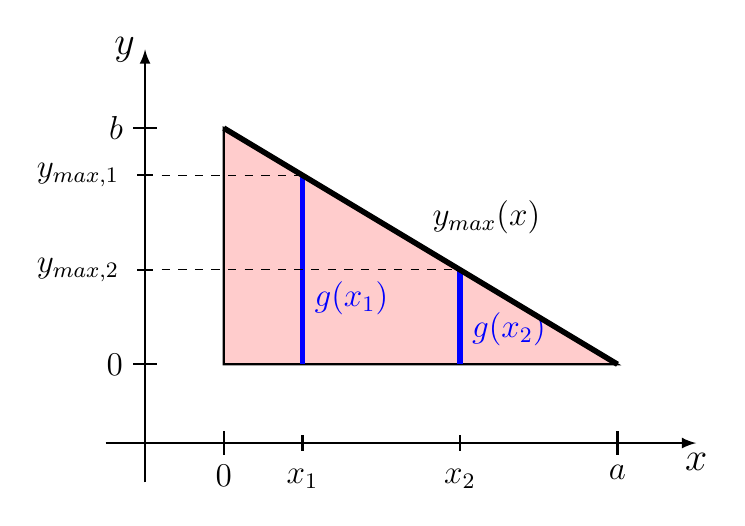
\begin{tikzpicture}[
        scale=1.0,
        >=latex, 
        font=\small\sffamily
    ]
    % --- Koordinaten-Definition ---
    \def\a{6} % Länge der Basis des Dreiecks
    \def\b{4} % Höhe des Dreiecks
    \def\k{0.6} % Steigung der Hypotenuse ((b-1)/(a-1))

    % Achsen-Endpunkte
    \coordinate (Origin) at (0,0);
    \coordinate (A) at (1,1);
    \coordinate (XEnd) at (\a+1,0);
    \coordinate (YEnd) at (0,\b+1);

    % --- Fläche füllen ---
    \fill[red!20] 
        (A) -- (\a,1) -- (1,\b) -- cycle;

    % --- Achsen zeichnen ---
    \draw[->, thick] (-0.5,0) -- (XEnd) node[below] {\Large $x$};
    \draw[->, thick] (0,-0.5) -- (YEnd) node[left] {\Large $y$};

    % --- Ticks und Labels X-Achse ---
    \draw[thick] (\a, -0.15) -- (\a, 0.15) node[below=0.3cm] {\large $a$};
    \draw[thick] (1, -0.15) -- (1, 0.15) node[below=0.3cm] {\large $0$};
    \draw[thick] (2, -0.1) -- (2, 0.1) node[below=0.3cm] {\large $x_1$};
    \draw[thick] (4, -0.1) -- (4, 0.1) node[below=0.3cm] {\large $x_2$};
    \draw[thick] (-0.1, \b-\k*1) -- (0.1, \b-\k*1) node[left=0.3cm] {\large $y_{\text{max},1}$};
    \draw[thick] (-0.1, \b-\k*3) -- (0.1, \b-\k*3) node[left=0.3cm] {\large $y_{\text{max},2}$};

    % --- Ticks und Labels Y-Achse ---
    \draw[thick] (-0.15, \b) -- (0.15, \b) node[left=0.3cm] {\large $b$};
    \draw[thick] (-0.15, 1) -- (0.15, 1) node[left=0.3cm] {\large $0$};

    % --- Das Dreieck als Linie zeichnen ---
    \draw[thick] (1,1) -- (\a,1) -- (1,\b) -- cycle;

    % --- blaue Linie von (2,1) nach (2, \b-\k*1) ---
    \draw[line width=2pt, blue] (2,1) -- (2,\b-\k*1) node[midway,pos=0.35, right] {\large $g(x_1)$};
    \draw[line width=2pt, blue] (4,1) -- (4,\b-\k*3) node[midway,pos=0.37, right] {\large $g(x_2)$};

    % --- strichlierte Linie von (0,g(x1)) nach (2,g(x1)) ---
    \draw[dashed, thin] (0,\b-\k*1) -- (2,\b-\k*1);
    \draw[dashed, thin] (0,\b-\k*3) -- (4,\b-\k*3);

    % --- Dicke Linie für y_max(x) ---
    \draw[line width=2pt] (\a,1) -- (1,\b) node[midway, above right] {\large $y_{\text{max}}(x)$};

    \end{tikzpicture}
    }
    \caption{Flächeninhalt eines Dreiecks mit den Eckpunkten $(0,0)$, $(a,0)$ und $(0,b)$. Der Flächeninhalt wird über ein Doppelintegral berechnet, wobei die Funktion $f(x,y) = 1$ gewählt wird. Man sieht, dass die obere Integrationsgrenze $y_{\text{max}}$ von $x$ abhängt.}\label{fig: flaeche_dreieck_doppelintegral}
\end{figure}


\subsection{Beispiel: Fläche eines Kreises}\label{subsec: flaeche_kreis}
Die Berechnung der Fläche eines Kreises mit Radius $R$ ist ein klassisches Beispiel, bei dem die Wahl des richtigen Koordinatensystems die Rechnung erheblich vereinfacht.
In kartesischen Koordinaten $(x,y)$ ist der Rand des Kreises durch die Gleichung $x^2 + y^2 = R^2$ gegeben. Dies führt in kartesischen Koordinaten auf Integrale über Wurzelterme ($\int \sqrt{R^2-x^2} \, \dd x$), die oft mühsam zu lösen sind.

Der Übergang zu \textbf{Polarkoordinaten} $(r, \varphi)$ bietet sich hier aufgrund der Symmetrie an.
Der Radius $r$ läuft von $0$ bis $R$ und der Winkel $\varphi$ deckt den Vollkreis von $0$ bis $2\pi$ ab.

\noindent \textbf{Aber Achtung:} Man darf beim Integrieren nicht einfach $\dd A = \dd r \cdot \dd \varphi$ setzen.

\subsubsection*{Das Flächenelement in Polarkoordinaten}
Um das korrekte Flächenelement $\dd A$ zu bestimmen, betrachten wir ein infinitesimal kleines Teilstück des Kreises im Abstand $r$ vom Ursprung (siehe \cref{fig: flaechenelemnt_polar}).
Dieses Teilstück wird durch eine kleine Änderung des Radius $\dd r$ und eine kleine Änderung des Winkels $\dd \varphi$ aufgespannt.
\begin{itemize}
    \item Die Seitenlänge in radialer Richtung ist einfach $\dd r$.
    \item Die Seitenlänge in tangentialer Richtung entspricht jedoch einer Bogenlänge. Da der Umfang eines Kreises mit dem Radius wächst, ist diese Bogenlänge abhängig von $r$. Sie beträgt $\dd s = r \cdot \dd \varphi$.
\end{itemize}
Das resultierende Flächenstück ist näherungsweise ein Rechteck mit den Seitenlängen $\dd r$ und $r \cdot \dd \varphi$.
\begin{equation}\label{eq: flaechenelement_polar}
    dA = \underbrace{\dd r}_{\text{Länge}} \cdot \underbrace{(r \cdot \dd \varphi)}_{\text{Breite}} = r \, \dd r \, \dd \varphi \mDot
\end{equation}
Der Faktor $r$ fungiert hier als Gewichtungsfaktor: Ein Winkelstück $\dd \varphi$ überstreicht weiter außen (großes $r$) im Kreis eine größere Fläche als nahe am Ursprung.

\begin{figure}[htb]
    \centering
    \begin{tikzpicture}[>=Stealth, scale=1.0]
            % Definitionen
            \def\R{3.5}
            \def\angA{30}
            \def\angB{60}
            \def\rIn{2.0}
            \def\rOut{2.9}
            \definecolor{boxcolOrange}{RGB}{255, 191, 77} % or use your preferred RGB values
            \definecolor{boxcolDarkOrange}{RGB}{255, 140, 0}

            % Koordinatensystem
            \draw[->, line width=1pt] (-0.5,0) -- (4,0) node[right] {$x$};
            \draw[->, line width=1pt] (0,-0.5) -- (0,4) node[above] {$y$};
            
            % Kreisbogen andeuten (gestrichelt)
            \draw[dashed, gray] (0,0) circle (\rOut);
            
            % Segment zeichnen (Flächenelement)
            \fill[fill=boxcolOrange] (\angA:\rIn) arc(\angA:\angB:\rIn) -- (\angB:\rOut) arc(\angB:\angA:\rOut) -- cycle;
            \draw[thick, fill=boxcolOrange] (\angA:\rIn) arc(\angA:\angB:\rIn) -- (\angB:\rOut) arc(\angB:\angA:\rOut) -- cycle;
            
            % Linien vom Ursprung
            \draw[thin] (0,0) -- (\angA:\rOut);
            \draw[thin] (0,0) -- (\angB:\rOut);
            
            % Beschriftungen
            % dr
            \draw[|<->|] (\angA-5:\rIn) -- (\angA-5:\rOut) node[midway,pos=0.6, below] {$\dd r$};
            
            % r dphi (Bogenlänge)
            \draw[<->] (\angA:\rIn+0.4) arc(\angA:\angB:\rIn+0.4) node[midway, above, rotate=-42] {$r \cdot \dd \varphi$};
            
            % r Vektor
            \draw[->, blue, line width=1.2pt] (0,0) -- (\angA:{\rIn+0.4}) node[midway, below right] {$r$};
            
            % Winkel dphi
            \draw[<->] (\angA:1.) arc(\angA:\angB:1.) node[midway, above right] {$\dd \varphi$};
            
            % dA Label
            \node[boxcolDarkOrange] at (45:4.2) {$\dd A = r \, \dd \varphi \, \dd r$};
            \draw[-, black, line width=0.5pt] (55:\rOut) -- (55:3.5);
    \end{tikzpicture}
    \caption{Geometrische Herleitung des Flächenelements in Polarkoordinaten. Die Fläche $dA$ spannt sich aus der radialen Änderung $\dd r$ und der Bogenlänge $r \cdot \dd \varphi$ auf.}\label{fig: flaechenelemnt_polar}
\end{figure}

\begin{rememberbox}{Flächenelement in Polarkoordinaten}
    Bei der Integration mit Polarkoordinaten darf der Radius $r$ im Integranden nicht vergessen werden. Das Flächenelement lautet:
    \begin{equation}
        dA = r \, \dd r \, \dd \varphi \mDot
    \end{equation}
    Anschaulich bedeutet dies: Je weiter man vom Mittelpunkt entfernt ist (größeres $r$), desto mehr Fläche entfällt auf denselben Winkelbereich $\dd \varphi$.
\end{rememberbox}
\textit{Anmerkung:} Formell wird das Flächenelement bei einer Koordinatentransformation über die Determinante der Jacobi-Matrix hergeleitet. Dies wird in fortgeschrittenen Mathematik- oder Physikkursen behandelt. 
\subsubsection*{Berechnung der Fläche}
Die Gesamtfläche $A$ des Kreises ergibt sich nun durch Integration über den gesamten Radius $R$ und den vollen Winkel $2\pi$:
\begin{equation}
    A = \int_{0}^{2\pi} \int_{0}^{R} \underbrace{r \, \dd r \, \dd \varphi}_{dA} \mDot
\end{equation}
Da die Grenzen für $r$ und $\varphi$ unabhängig voneinander sind, können die Integrale getrennt berechnet werden:
\begin{align}
    A &= \left( \int_{0}^{2\pi} \dd \varphi \right) \cdot \left( \int_{0}^{R} r \, \dd r \right) \\
      &= \bigg[ \varphi \bigg]_{0}^{2\pi} \cdot \bigg[ \frac{1}{2}r^2 \bigg]_{0}^{R} \\
      &= (2\pi - 0) \cdot \left( \frac{1}{2}R^2 - 0 \right) \\
      &= 2\pi \cdot \frac{1}{2}R^2 = \pi R^2 \mDot
\end{align}
Somit erhalten wir die bekannte Formel für die Kreisfläche:
\begin{equation}
    A = \pi R^2 \mDot
\end{equation}


\subsection{Dreidimensionales Integral (Volumenintegral)}\label{sec: Dreidimensionales_Integral}
Das dreidimensionale Integral, auch Volumenintegral genannt, wird beispielsweise verwendet, um Volumina in dreidimensionalen Räumen zu berechnen, indem auch hier die Funktion $f(x,y,z) = 1$ gewählt wird und über den Definitionsbereich $D$ integriert wird. 

Im Allgemeinen (für ein beliebiges $f(x,y,z)$) ist das Volumenintegral über dem Bereich $D: [a,b] \times [c,d] \times [e,f]$ definiert als
\begin{equation}
    \iiint_{V} f(x,y,z) \,\dd V = \int_{a}^{b} \int_{c}^{d} \int_{e}^{f} f(x,y,z) \,\dd z \,\dd y \,\dd x \mDot
\end{equation}

Möchte man das Volumen eines dreidimensionalen Körpers berechnen, so wird die Funktion $f(x,y,z) = 1$ gewählt, und das Volumen $V$ wird bestimmt über
\begin{equation}
    V = \iiint_{V} 1 \,\dd V = \iiint_{V} \,\dd V \mDot
\end{equation}

\subsubsection{Volumenelement in Kugelkoordinaten}
In vielen Fällen, insbesondere bei kugelsymmetrischen Problemen, ist es sinnvoll, von kartesischen Koordinaten $(x,y,z)$ in \textbf{Kugelkoordinaten} $(r, \theta, \varphi)$ zu wechseln. Hierbei bezeichnet $r$ den Abstand vom Ursprung, $\theta$ den Polarwinkel (Winkel zur $z$-Achse) und $\varphi$ den Azimutalwinkel (Winkel in der $xy$-Ebene von der $x$-Achse aus gemessen). 

Der Vollständigkeit halber wollen wir auch hier das Volumenelement in Kugelkoordinaten angeben.
\begin{rememberbox}{Volumenelement in Kugelkoordinaten}
    Bei der Integration mit Kugelkoordinaten lautet das Volumenelement:
    \begin{equation}
        \dd V = r^2 \sin(\theta) \, \dd r \, \dd \theta \, \dd \varphi \mDot
    \end{equation}
    Ein Faktor $r$ kommt aus dem Flächenelement von Polarkoordinaten und ein zusätzlicher Faktor $r \sin(\theta)$ berücksichtigt die Zunahme der Kreisumfangslänge in Abhängigkeit von $r$ und $\theta$. Damit wird die Geometrie der Kugelkoordinaten gewahrt und sichergestellt, dass das Volumenelement korrekt skaliert wird.
\end{rememberbox}
\begin{figure}[htb]
    \centering
    \includegraphics[width=0.4\linewidth]{Bilder/Kapitel_MathematischeEinschuebe/Kugelkoordinaten_erklaerung.png}
    \caption{Kugelkoordinaten $(r, \theta, \varphi)$ im dreidimensionalen Raum. Der Winkel $\varphi$ bezeichnet den Azimutalwinkel in der $xy$-Ebene von der $x$-Achse aus gemessen und der Winkel $\theta$ den Polarwinkel zur $z$-Achse.}\label{fig: kugelkoordinaten}
\end{figure}
\newpage

\chapter{Differentialgleichungen}\label{chap: differentialgleichungen}
Eine \textbf{Differentialgleichung} (DGL) ist eine mathematische Gleichung, die eine oder mehrere Funktionen und ihre Ableitungen enthält. Im Wesentlichen beschreibt eine DGL die Beziehung zwischen einer sich ändernden Größe und ihrer Änderungsrate.

Stellen wir uns eine Funktion $f(x)$ vor. Eine DGL verknüpft $x$, $f(x)$, die erste Ableitung $f'(x) = \frac{\dd f}{\dd x}$, die zweite Ableitung $f''(x) = \frac{\dd^2 f}{\dd x^2}$ und so weiter.

\subsubsection{Bedeutung von Differentialgleichungen}
Differentialgleichungen sind das Herzstück vieler wissenschaftlicher und technischer Disziplinen. Sie ermöglichen es uns, dynamische Prozesse zu modellieren, bei denen sich Größen im Laufe der Zeit oder im Raum ändern. Anwendungsgebiete sind vielfältig:
\begin{itemize}
    \item \textbf{Physik:} Bewegung von Objekten, Schwingungen, Wärmeleitung, Quantenmechanik.
    \item \textbf{Ingenieurwesen:} Regelungstechnik, elektrische Schaltkreise, Strömungsdynamik.
    \item \textbf{Biologie:} Populationswachstum, Ausbreitung von Krankheiten.
    \item \textbf{Wirtschaft:} Finanzmodelle, Marktdynamiken.
\end{itemize}

\subsubsection{Klassifizierung von Differentialgleichungen}
Man klassifiziert DGLs nach drei Hauptkriterien:

\begin{enumerate}
    \item \textbf{Gewöhnlich vs. Partiell:}
    \begin{itemize}
        \item \textbf{Gewöhnliche Differentialgleichungen (GDGL):} Enthalten nur Funktionen einer einzigen unabhängigen Variable und deren Ableitungen. Beispiel: $f'(x) + 2f(x) = \sin(x)$.
        \item \textbf{Partielle Differentialgleichungen (PDGL):} Enthalten Funktionen von mehreren unabhängigen Variablen und deren partielle Ableitungen.
    \end{itemize}
    \item \textbf{Ordnung:} Die Ordnung einer DGL ist die Ordnung der höchsten vorkommenden Ableitung.
    \begin{itemize}
        \item DGL 1. Ordnung: $f'(x) + 3 f(x) = 0$.
        \item DGL 2. Ordnung: $f''(x) + 4f'(x) + 3f(x) = x^2$.
    \end{itemize}
    \item \textbf{Linearität:} Eine DGL ist linear, wenn die gesuchte Funktion und ihre Ableitungen nur in der ersten Potenz und nicht miteinander multipliziert vorkommen.
\end{enumerate}

\section{Beispiel aus der Physik: Bewegung}
Ein klassisches Beispiel zur Veranschaulichung ist die geradlinige Bewegung eines Objekts entlang einer Dimension -- somit kann man das Problem mit Skalaren beschreiben, ohne Vektoren. Die physikalischen Größen Ort, Geschwindigkeit und Beschleunigung sind durch Ableitungen miteinander verknüpft.

Sei $s(t)$ der Ort eines Objekts zur Zeit $t$.
\begin{itemize}
    \item Die \textit{Geschwindigkeit} $v(t)$ ist die erste Ableitung des Ortes nach der Zeit:
    $$ v(t) = s'(t) = \frac{\dd s}{\dd t} $$
    \item Die \textit{Beschleunigung} $a(t)$ ist die erste Ableitung der Geschwindigkeit bzw. die zweite Ableitung des Ortes nach der Zeit:
    $$ a(t) = v'(t) = s''(t) = \frac{\dd v}{\dd t} = \frac{\dd^2 s}{\dd t^2} $$
\end{itemize}

\subsection{Fall 1: Konstante Beschleunigung}
Betrachten wir den freien Fall (ohne Luftwiderstand). Die Beschleunigung $a(t) = \const$ ist konstant und entspricht der Erdbeschleunigung $a = g \approx \SI{9.81}{\meter\per\second\squared}$. Nehmen wir an, die positive Richtung sei nach unten.
Die DGL für die Geschwindigkeit lautet:
$$ v'(t) = g $$
Dies ist eine sehr einfache DGL. Wir lösen sie durch direkte Integration:
$$ \int v'(t) \, \dd t = \int g \, \dd t \implies v(t) = g \cdot t + C_1 $$
Die Integrationskonstante $C_1$ ist die Anfangsgeschwindigkeit $v(0)$. Also:
$$ v(t) = g \cdot t + v_0 $$
Um nun den Ort $s(t)$ zu finden, lösen wir die DGL $s'(t) = v(t)$:
$$ s'(t) = g \cdot t + v_0 $$
Nochmalige Integration liefert:
$$ \int s'(t) \, \dd t = \int (g \cdot t + v_0) \, \dd t \implies s(t) = \frac{1}{2}g \cdot t^2 + v_0 \cdot t + C_2 $$
Die Integrationskonstante $C_2$ ist der Anfangsort $s(0)$, also $s_0$. Das Ergebnis ist die bekannte Formel für die gleichmäßig beschleunigte Bewegung:
$$ s(t) = \frac{1}{2}gt^2 + v_0 t + s_0 $$

\section{Lösungsmethoden für DGLs 1. Ordnung}
Die Lösung einer DGL ist eine Funktion, die die Gleichung erfüllt. Oft gibt es eine ganze Schar von Lösungen (abhängig von Integrationskonstanten). Eine eindeutige Lösung erhält man durch Angabe von \textbf{Anfangs- oder Randbedingungen} (\zB $f(x_0) = f_0 = 4.2$).

\subsection{Trennung der Variablen}
Eine der grundlegendsten Methoden ist die Trennung der Variablen. Sie ist anwendbar, wenn sich die DGL in die Form
$$ y' = f(x) \cdot g(y) $$
bringen lässt. Man schreibt $y' = \frac{\dd y}{\dd x}$ und "trennt" dann die Variablen $x$ und $y$ auf unterschiedliche Seiten der Gleichung:
$$ \frac{\dd y}{g(y)} = f(x) \, \dd x $$
Anschließend integriert man beide Seiten:
$$ \int \frac{\dd y}{g(y)} = \int f(x) \, \dd x + C $$

\subsubsection{Beispiel: Radioaktiver Zerfall}
Die Zerfallsrate eines radioaktiven Materials ist proportional zur vorhandenen Menge $N(t)$.
$$ N'(t) = -\lambda \cdot N(t) \quad (\lambda > 0 \text{ ist die Zerfallskonstante}) $$
Wir trennen die Variablen:
$$ \frac{\dd N}{N} = -\lambda \, \dd t $$
Integration beider Seiten:
$$ \int \frac{1}{N} \, \dd N = \int -\lambda \, \dd t $$
$$ \ln|N| = -\lambda t + C $$
Um $N$ zu isolieren, wenden wir die Exponentialfunktion an:
$$ |N| = e^{-\lambda t + C} = e^C \cdot e^{-\lambda t} $$
Da $N$ eine Menge ist ($N>0$) und $e^C$ eine positive Konstante ist, können wir dies als $N_0 = e^C$ (die Anfangsmenge bei $t = 0$) schreiben.
$$ N(t) = N_0 \cdot e^{-\lambda t} $$

\section{Ausblick: DGLs höherer Ordnung}
Lineare Differentialgleichungen zweiter Ordnung mit konstanten Koeffizienten haben die Form:
$$ a\cdot y'' + b\cdot y' + c\cdot y = 0 $$
Der Lösungsansatz hierfür ist $y(x) = e^{rx}$. Setzt man diesen Ansatz in die DGL ein, erhält man die \textbf{charakteristische Gleichung}:
$$ ar^2 + br + c = 0 $$
Die Lösungen dieser quadratischen Gleichung für $r$ bestimmen die Form der allgemeinen Lösung für $y(x)$. Dies ist ein grundlegendes Konzept in der Analyse von Schwingungssystemen (mechanisch oder elektrisch).

% Chapter end - always start new page after chapter
\newpage